%---------------------------------------------------------------------------------------
%	PACKAGES AND THEMES
%---------------------------------------------------------------------------------------
\documentclass[aspectratio=169,xcolor=dvipsnames,handout]{beamer} % handout

\newcommand{\backupbegin}{
   \newcounter{finalframe}
   \setcounter{finalframe}{\value{framenumber}}
}
\newcommand{\backupend}{
   \setcounter{framenumber}{\value{finalframe}}
}

\newcommand\T{\rule{0pt}{2.6ex}}       % Top strut
\newcommand\B{\rule[-1.2ex]{0pt}{0pt}} % Bottom strut

\usepackage{array}
\newcolumntype{P}[1]{>{\centering\arraybackslash}p{#1}}
\newcolumntype{M}[1]{>{\centering\arraybackslash}m{#1}}

\usetheme{SimplePlus}

\usepackage{xcolor}
\usepackage{hyperref}
\usepackage{graphicx} % Allows including images/logos
\usepackage{booktabs} % Allows the use of \toprule, \midrule and \bottomrule in tables
\usepackage{comment}
\usepackage{tikz}
\usepackage{mhchem}
\usepackage{setspace}
\usepackage{array}
\newcolumntype{L}[1]{>{\raggedright\let\newline\\\arraybackslash\hspace{0pt}}m{#1}}
\newcolumntype{C}[1]{>{\centering\let\newline\\\arraybackslash\hspace{0pt}}m{#1}}
\newcolumntype{R}[1]{>{\raggedleft\let\newline\\\arraybackslash\hspace{0pt}}m{#1}}
\usepackage{setspace}
\usepackage{amsmath}
\usepackage{siunitx}
\sisetup{detect-all}
\usepackage{pifont}
\newcommand{\xmark}{\ding{55}}
\usepackage{svg}
\usepackage[absolute,overlay]{textpos}
\usepackage{bm}

\newcommand{\greencheck}{{\color{ForestGreen}\checkmark}}
\newcommand{\redcross}{{\color{Red}\xmark}}

% all pages logos
\logo{
    \begin{picture}(0,0)
        \put(0,0){\makebox(-60,235)[rt]{\includesvg[width=1cm]{images/logos/unibg_logo_single.svg}}}
         \put(0,0){\makebox(-25,235)[rt]{
\includegraphics[width=0.7cm]{images/logos/gaps.png}}}
    \end{picture}
}

\setbeamercovered{transparent}
\setbeamertemplate{footline}[frame number]{}


%---------------------------------------------------------------------------------------
%	TITLE PAGE
%---------------------------------------------------------------------------------------

\title[]{\large{Characterisation of the readout electronics of the Si(Li) tracker\\ for the first flight of the GAPS experiment}} % The short title appears at the bottom of every slide, the full title is only on the title page

\author[Luca Ghislotti] {Luca Ghislotti\\Master Thesis Defence\\ \vspace{0.3cm}\small September $30^{\text{th}}$, 2022}

\institute[UniBG]{
    \\Supervisor: prof. Massimo Manghisoni \\
    Co-Supervisors: Ph.D. Elisa Riceputi, M.Sc. Paolo Lazzaroni
}

\date{Computer Engineering\\Academic Year 2021/2022} % Date

% title page logos
\titlegraphic { 
    \begin{picture}(0,0)
        % VERSION WITH UNIBG AND GAPS LOGOS
        \put(25,164){\makebox(0,0)[rt]{
\includegraphics[width=4cm]{images/logos/unibg-logo.png}}}
        \put(90,170){\makebox(0,0)[rt]{
\includegraphics[width=1.4cm]{images/logos/gaps.png}}}
    \end{picture}
}


\begin{document}

%---------------------------------------------------------------------------------------
%	TITLE PAGE
%---------------------------------------------------------------------------------------

\frame[plain]{
    \vspace{-0.5cm}
    \titlepage
}


%---------------------------------------------------------------------------------------
%	General AntiParticle Spectrometer (GAPS)
%---------------------------------------------------------------------------------------

\begin{frame}{General AntiParticle Spectrometer (GAPS)}
\fontsize{9pt}{1}\selectfont
   \begin{columns}
   \vspace{0.05cm}
    \column{0.58\textwidth}
        \pause
        \vskip0.2cm
        GAPS is an \textbf{Antarctic balloon experiment} designed to detect low-energy cosmic antinuclei as an indirect signature of \textbf{Dark Matter}\pause

        \vspace{0.3cm}
        \textbf{\large \textcolor{ForestGreen}{The instrument}}\\
        \vspace{0.25cm}
        \textbf{\textcolor{Red}{Time-of-Flight System (TOF)}}
        \begin{itemize}
            \item 220 plastic scintillator paddles with Si-PM readout
        \end{itemize}\pause
        \vspace{0.15cm}
        \textbf{\textcolor{Red}{Si(Li) Tracker}}
        \begin{itemize}
            \item About 1000 lithium-drifted silicon (Si(Li)) detectors
            \item 10 layers with 10 cm spacing
            \item 12x12 Si(Li) detectors per layer
            \item Modular structure (360 modules)
        \end{itemize}\pause

        \vspace{0.25cm}
        The experiment is developed by an international collaboration that includes Japanese, US and Italian institutes, and it is funded by \textbf{NASA}, \textbf{INFN}, \textbf{ASI} and \textbf{JAXA}\pause
        
        \vspace{0.2cm}
        The \textbf{first flight} is scheduled for late 2023 from McMurdo National Science Foundation (NSF) Station in Antarctica
        
    \column{0.38\textwidth}
        \begin{figure}
        \centering
        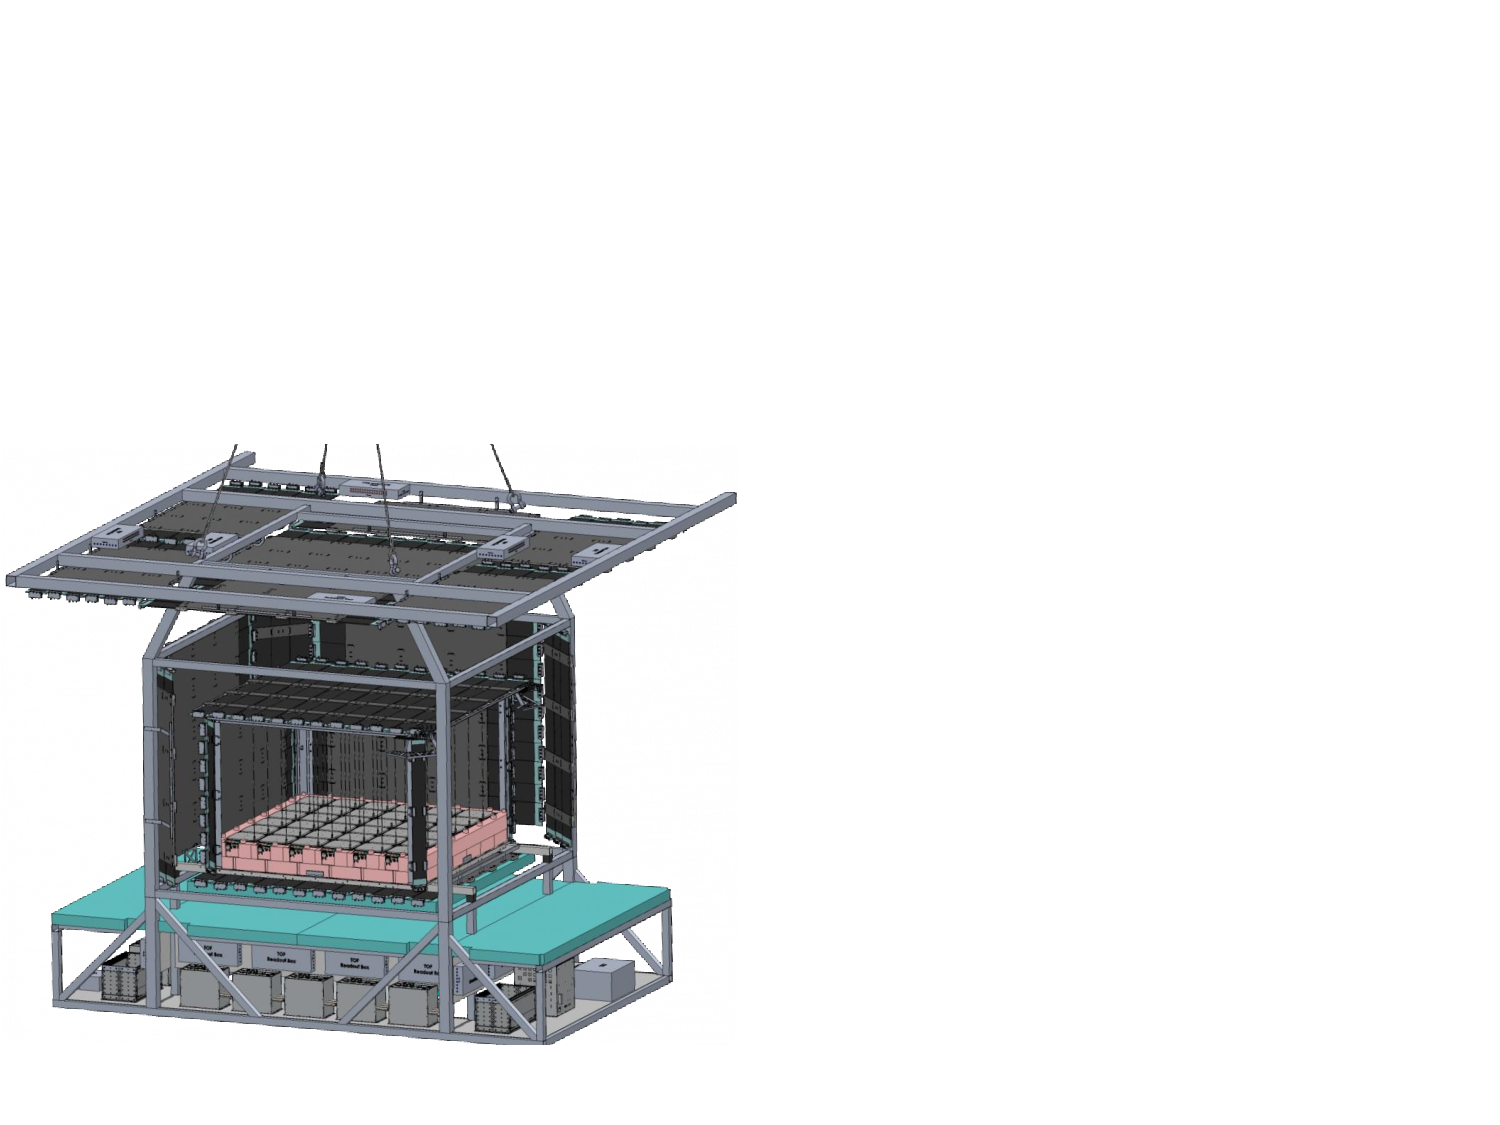
\includegraphics[width=0.95\textwidth]{images/experiment_intro/tracker_menjiao.pdf}
        \end{figure}
        \centering
        
\includegraphics[width=0.8\textwidth]{images/logos/loghi_presentazione.pdf}
    \end{columns}
\end{frame}


%---------------------------------------------------------------------------------------
%	Si(Li) tracker structure
%---------------------------------------------------------------------------------------

\begin{frame}{Si(Li) tracker structure}
    \fontsize{9pt}{1}\selectfont
    \settowidth{\leftmargini}{\usebeamertemplate{enumerate item}}
    \addtolength{\leftmargini}{\labelsep}
    \vspace{0.1cm}
    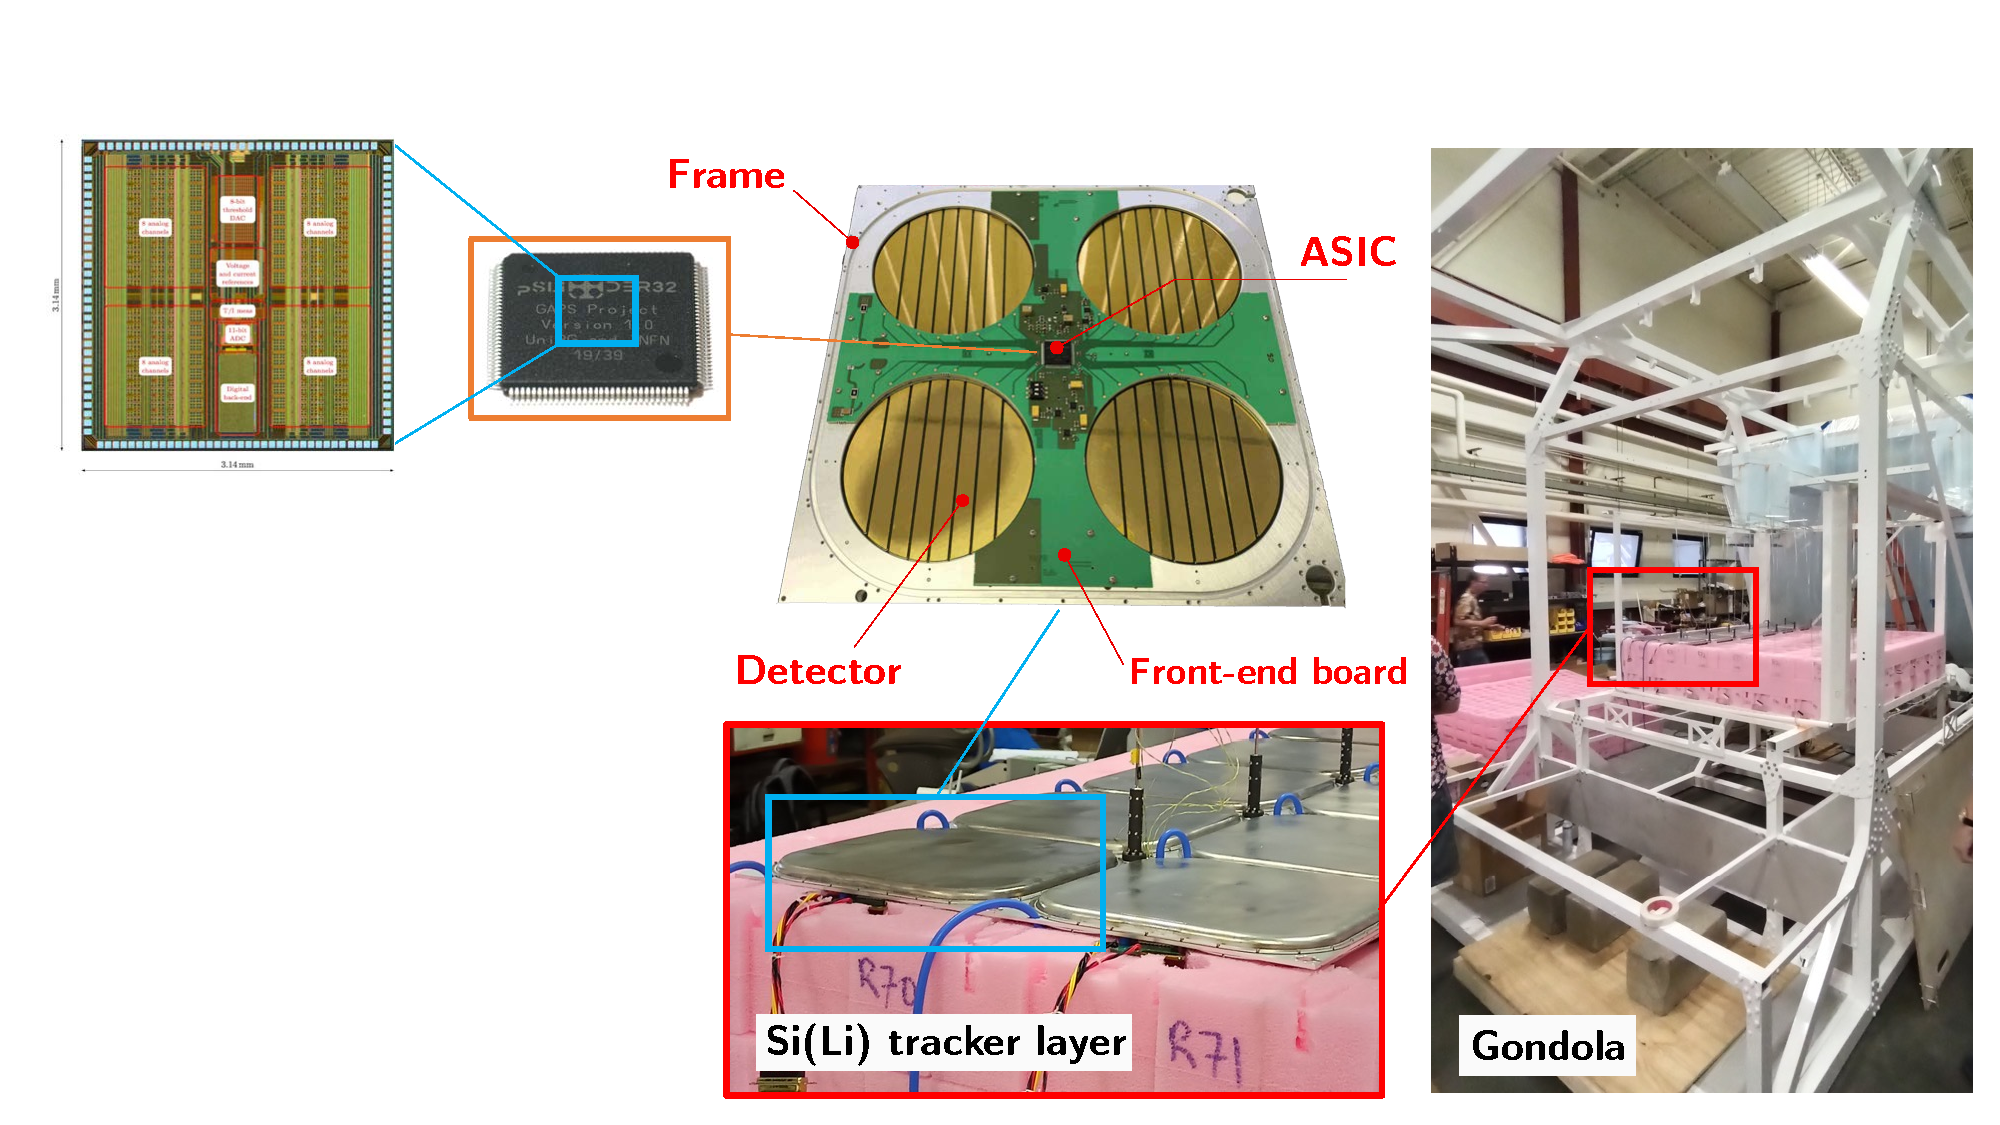
\includegraphics[width=0.99\textwidth]{images/experiment_intro/manghisoni_SIE_ASSEMBLY.pdf}

    \pause
    \begin{textblock*}{0.35\textwidth}(0.5cm, 4.2cm)
        \textbf{\textcolor{ForestGreen}{Module}}
        \fontsize{8.5pt}{1}\selectfont
        \vspace{0.05cm}
        \begin{itemize}
            \item 1 readout ASIC
            \item 1 Front-End Board (FEB)
            \item 4 Si(Li) detectors (8 strips each)
        \end{itemize}\pause
        \vspace{0.1cm}
        \fontsize{9pt}{1}\selectfont
        \textbf{\textcolor{ForestGreen}{Front-end electronics requirements}}
        \fontsize{8.5pt}{1}\selectfont
        \vspace{0.05cm}
        \begin{itemize}
            \item Channels per ASIC: \textbf{32}
            \item Operating temperature: \textbf{\SI{-40}{\celsius}}
            \item Power dissipation: $\leq$ \textbf{\SI{10}{\milli\watt/ch}}
            \item Dynamic range: \textbf{\SI{10}{\kilo\electronvolt} - \SI{100}{\mega\electronvolt}}
            \item Analog resolution: \textbf{\SI{4}{\kilo\electronvolt} (FWHM)}
            \item Threshold: \textbf{\SI{20}{\kilo\electronvolt}}
        \end{itemize}
    \end{textblock*}
\end{frame}


%---------------------------------------------------------------------------------------
%	SOMMARIO
%---------------------------------------------------------------------------------------

% SOMMARIO
\begin{frame}{Thesis work: overview}
    \settowidth{\leftmargini}{\usebeamertemplate{enumerate item}}
    \addtolength{\leftmargini}{\labelsep}
    \begin{columns}
        \column{0.6\textwidth}
        \fontsize{11pt}{1}\selectfont
        %\tableofcontents
        \pause
        \begin{enumerate}
            \setlength\itemsep{1em}
            \fontsize{10pt}{1}\selectfont
            \item \textbf{Evaluation of temperature effects on ASIC performance}
            \begin{itemize}
                \fontsize{8.5pt}{1}\selectfont
                \setlength\itemsep{0.3em}
                \item Current reference
                \item Input-output channel trans-characteristic
                \item Global threshold voltage
                \item Equivalent Noise Charge (ENC) at \SI{-40}{\celsius}
            \end{itemize}\pause
            \fontsize{10pt}{1}\selectfont
            \item \textbf{Si(Li) tracker flight components validation}
            \begin{itemize}
                \fontsize{8.5pt}{1}\selectfont
                \setlength\itemsep{0.3em}
                \item Front-End Boards (FEBs)
                \item Dummy-1 front-end boards
                \item Flex-rigid boards
                \item Connectors for termination
                \item Front-end board shields
            \end{itemize}\pause
            \fontsize{10pt}{1}\selectfont
            \item \textbf{X-ray and particle detection with an assembled Si(Li) tracker module}
            \begin{itemize}
                \fontsize{8.5pt}{1}\selectfont
                \setlength\itemsep{0.3em}
                \item X-ray detection with an Americium 241 source
                \item Cosmic muon detection using an external scintillator
            \end{itemize}
        \end{enumerate}
        \column{0.3\textwidth}
        \centering
        \vskip0.1cm
        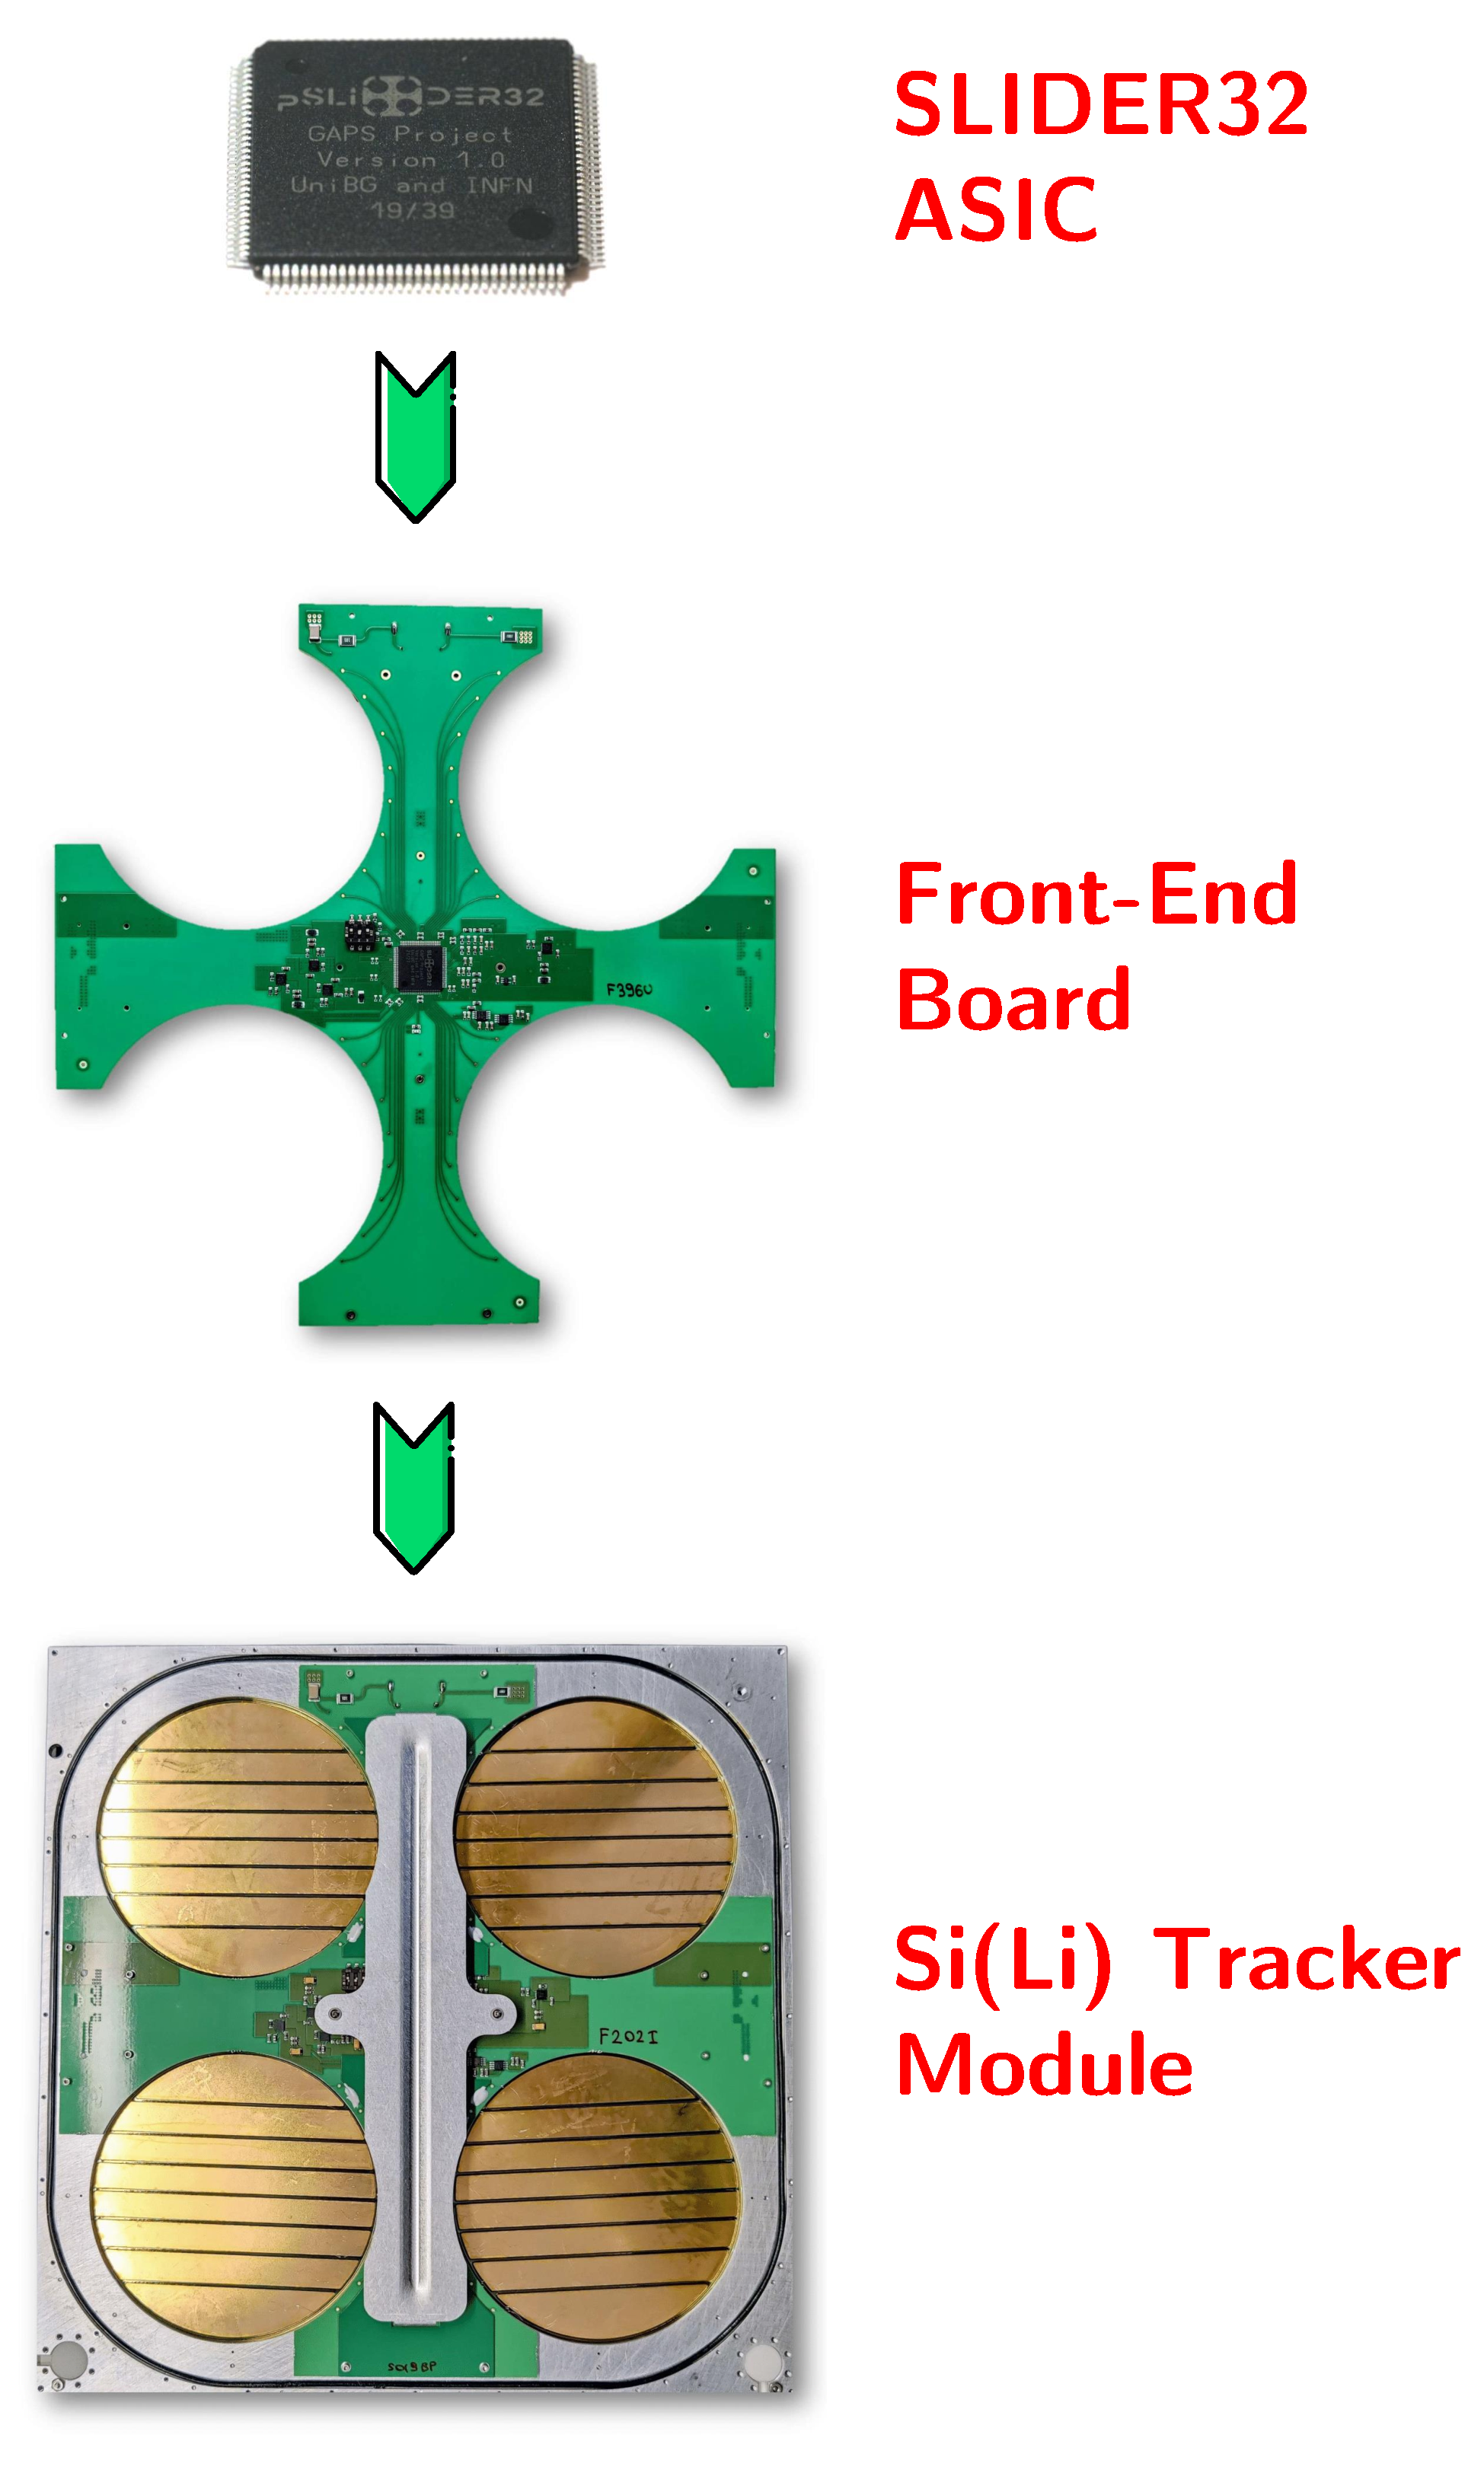
\includegraphics[height=0.85\textheight]{images/random/workflow.pdf}
    \end{columns}
\end{frame}


%---------------------------------------------------------------------------------------
%	ASIC characterisation at different temperatures
%---------------------------------------------------------------------------------------   

\begin{frame}{ASIC characterisation at different temperatures}
\fontsize{8.5pt}{1}\selectfont
    \begin{columns}[T]
    \column{0.475\textwidth}
        \vskip0.3cm
        \textbf{SLIDER32 ASIC test setup}\\
        \vskip0.15cm
        
        Tests conducted on the SLIDER32 readout ASIC with a purposely designed test board were aimed at evaluate temperature effects on:
        \begin{enumerate}
            \item Bandgap reference current
            \item Channel input-output characteristic
            \item DAC for setting the global threshold voltage
        \end{enumerate}

        \vskip0.05cm
        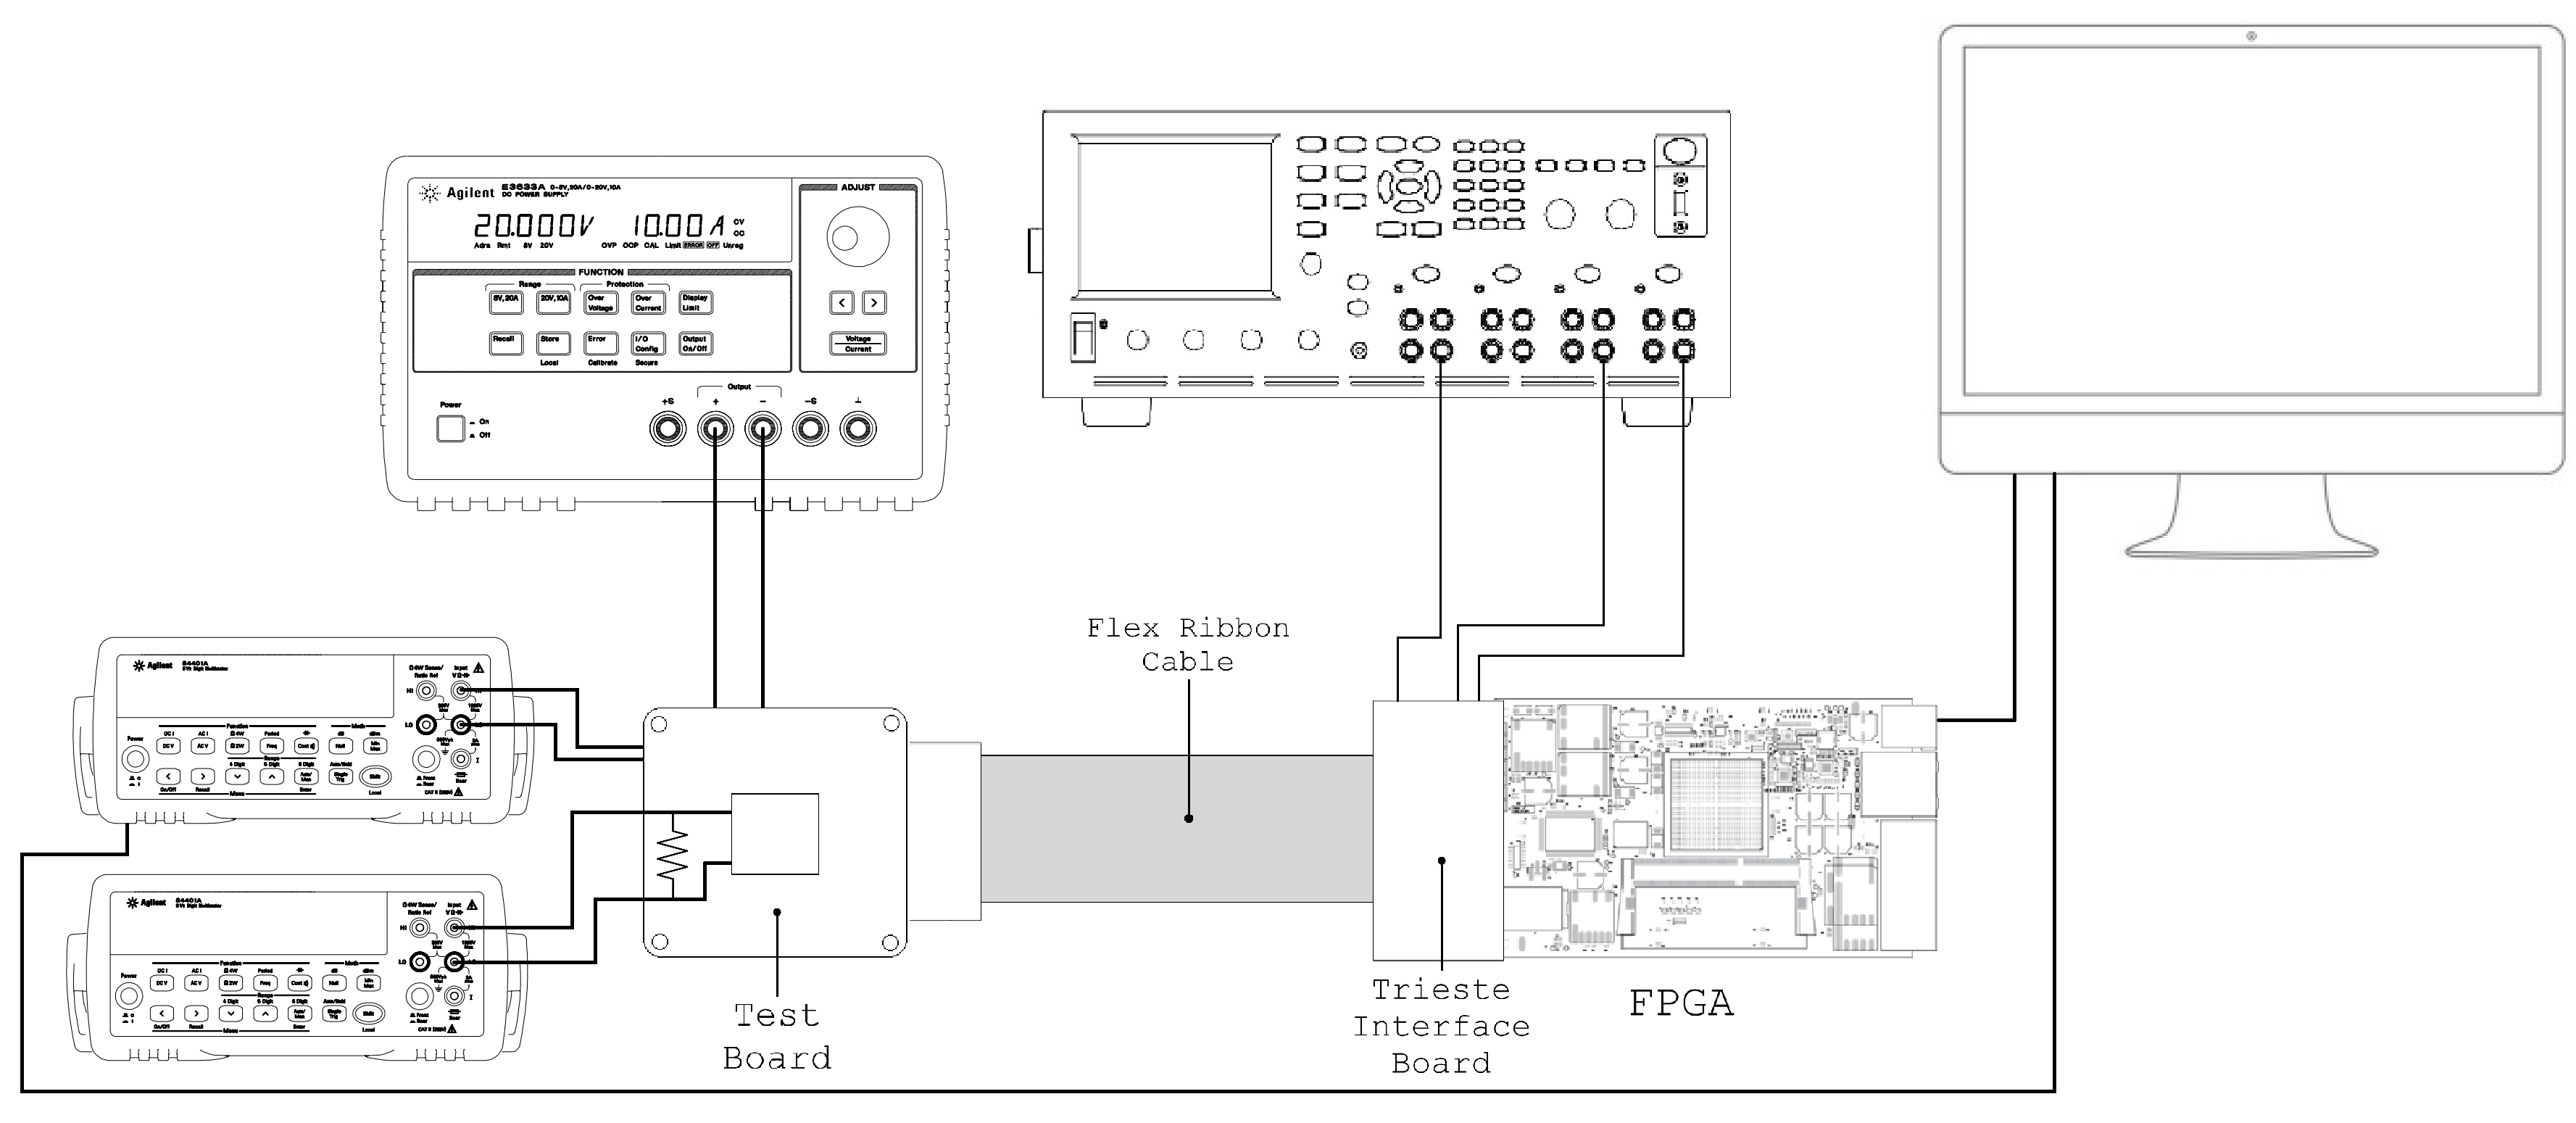
\includegraphics[width=0.95\textwidth]{images/temperature_effects/test_setup_test_board_csavrefgm_530mv.png}
        \vskip0.2cm

        Temperature range: 
        \begin{itemize}
            \item $\SI{-40}{\celsius} \div +\SI{30}{\celsius}$ with \SI{10}{\celsius} steps
            \item $\SI{-40}{\celsius} \div \SI{-30}{\celsius}$ with \SI{2}{\celsius} steps
        \end{itemize}

    \subsection{Bandgap reference current}
    \column{0.475\textwidth}
        \settowidth{\leftmargini}{\usebeamertemplate{itemize item}}
        \addtolength{\leftmargini}{\labelsep}
        \vskip0.3cm
        \textbf{Bandgap reference current}\\
        \vskip0.15cm
    
        Adjustable current reference by means of 3 bits (\texttt{BBB}) and \SI{5}{\micro\ampere} nominal value

        \vskip-0.4cm
        \begin{center}
            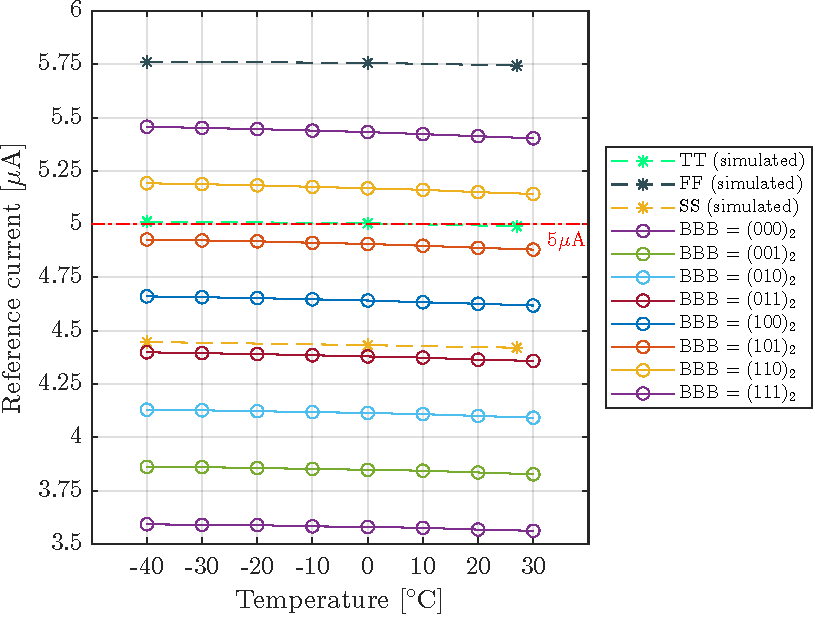
\includegraphics[height=0.48\textheight]{images/temperature_effects/BGR_current_Xtemp_all-BBB.pdf}
        \end{center}

        \vskip-0.2cm
        \begin{itemize}
            \item \SI{5}{\micro\ampere} nominal value obtained with \texttt{BBB} = $(\texttt{101})_{2}$ \greencheck
            \item $< \SI{1}{\percent}$ variation over the whole temperature range \greencheck
            \item $\thicksim \SI{1.8}{\micro\ampere}$ range @ \SI{-40}{\celsius} by adjusting \texttt{BBB} bits \greencheck
        \end{itemize}
    \end{columns}
\end{frame}


%---------------------------------------------------------------------------------------
%	Channel input-output characteristic
%---------------------------------------------------------------------------------------

\begin{frame}{Channel input-output characteristic}
\fontsize{8.5pt}{1}\selectfont
    \begin{columns}
    \column{0.375\textwidth}
        \settowidth{\leftmargini}{\usebeamertemplate{itemize item}}
        \addtolength{\leftmargini}{\labelsep}

        \vspace{-0.25cm}
        \begin{center}
             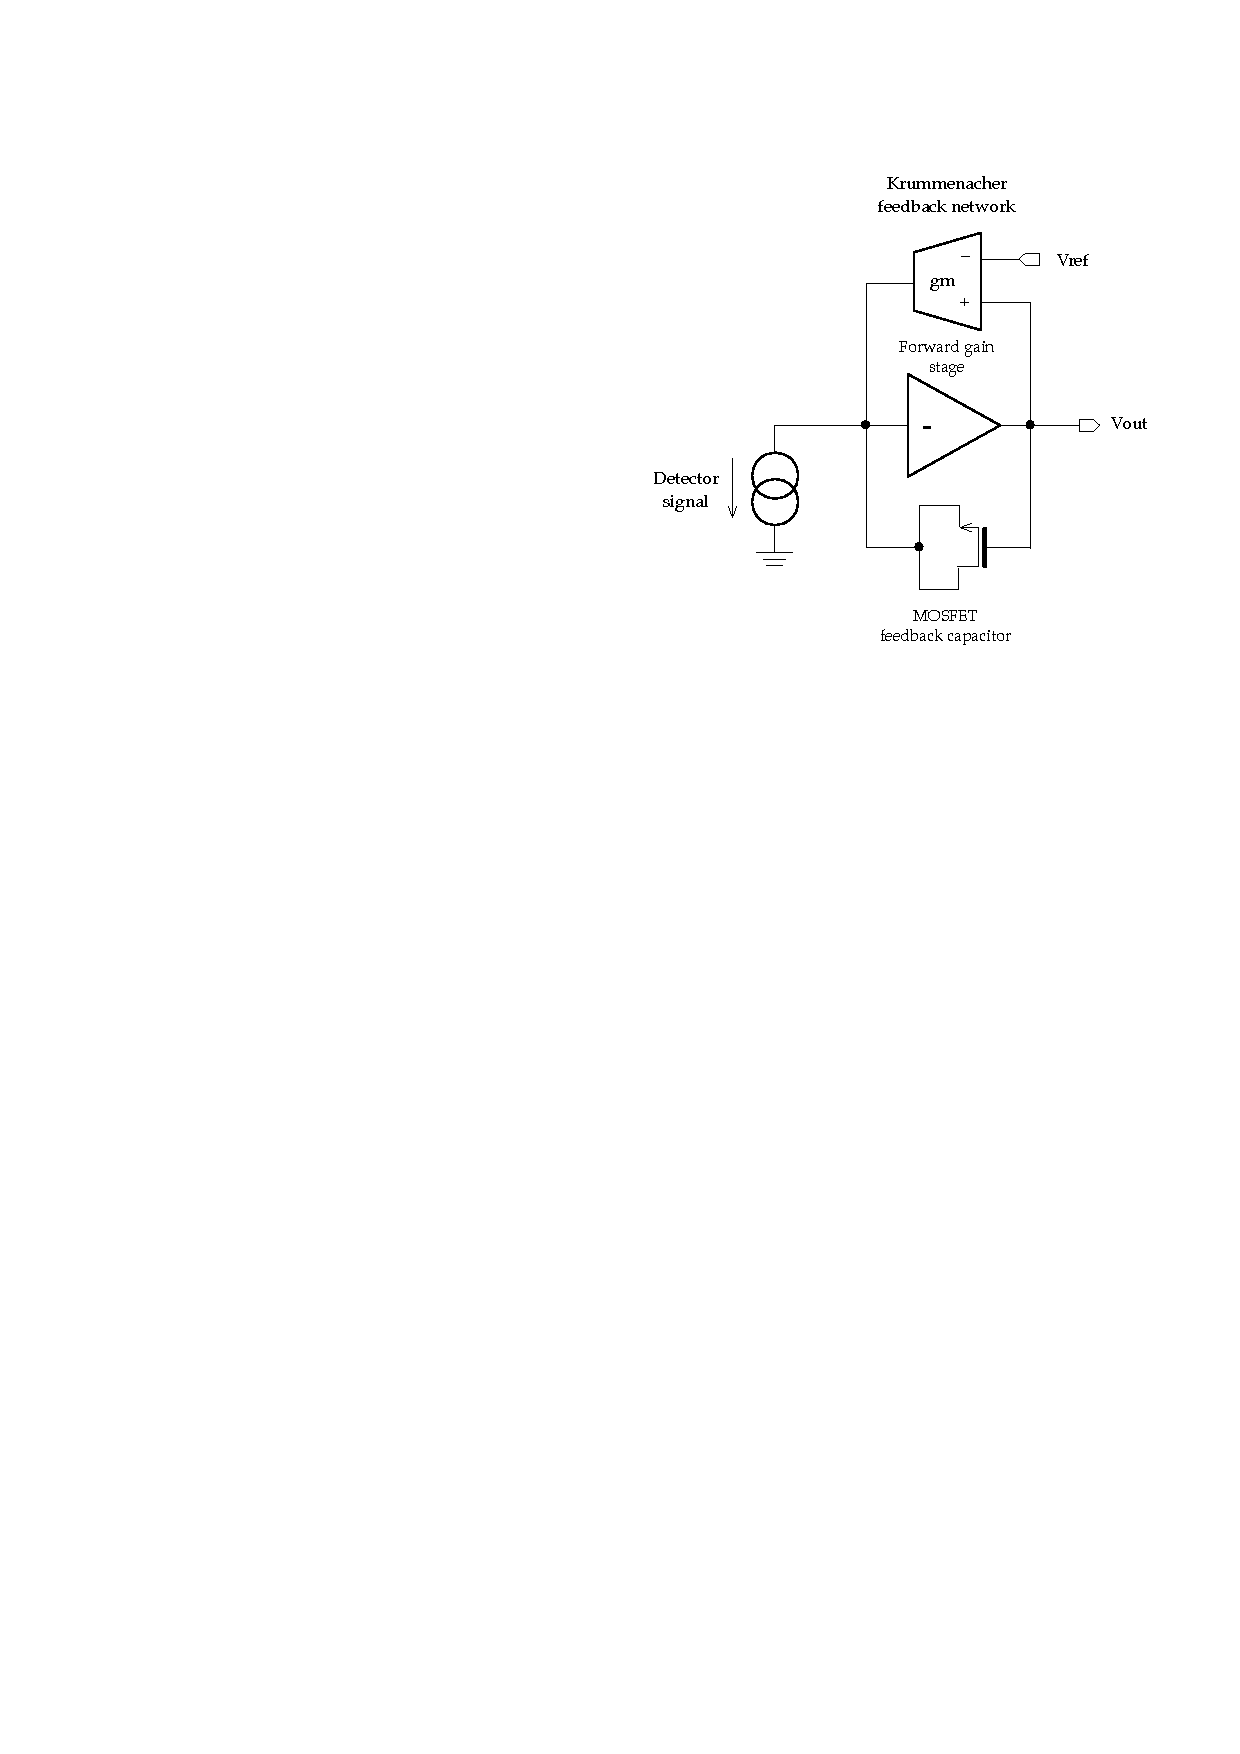
\includegraphics[height=0.55\textheight]{images/temperature_effects/CSA_schematic.pdf}
        \end{center}

        \vskip-0.2cm
        \begin{itemize}
            \item Charge Sensitive Amplifier (CSA) based on an inverting gain stage and a feedback capacitor
            \item \textbf{Dynamic signal compression} achieved by implementing the feedback capacitor with an NMOSFET
        \end{itemize}

        \column{0.6\textwidth}
            \settowidth{\leftmargini}{\usebeamertemplate{itemize item}}
            \addtolength{\leftmargini}{\labelsep}
            \vskip0.3cm
            \textbf{\texttt{CSAVrefGM} voltage: automatically regulated vs fixed to \SI{530}{\milli\volt}}\\
    
            \vskip-0.4cm
            \begin{center}
                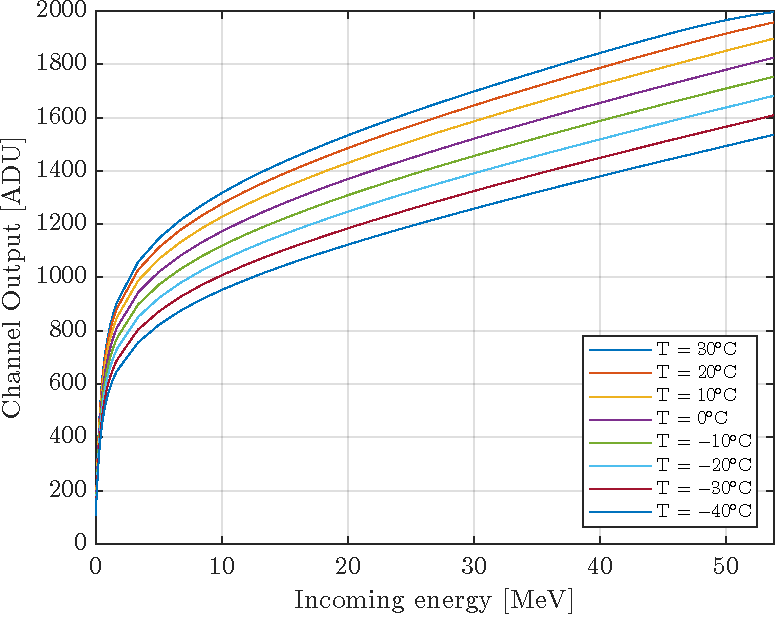
\includegraphics[height=0.37\textheight]{images/temperature_effects/fdt_csavrefgm_auto_tau6_keV_0011.pdf}
                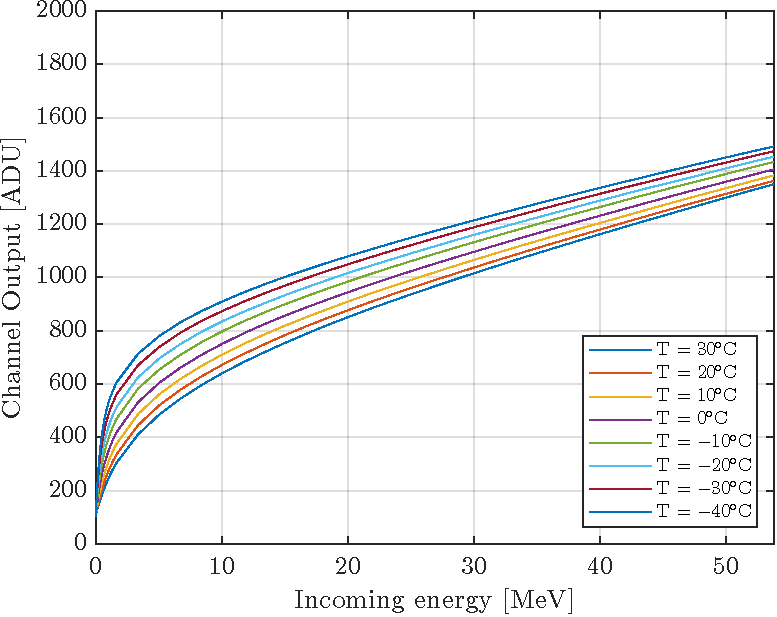
\includegraphics[height=0.37\textheight]{images/temperature_effects/fdt_csavrefgm_530mV_tau6_keV.pdf}
            \end{center}
    
            \vskip-0.2cm
            \begin{itemize}
                \item Both configurations successfully tested \greencheck
                \item Peaking time \#4: $\tau_{p} = \SI{0.98}{\micro\second}$, \texttt{TTT} bits set to $(\texttt{100})_{2}$
                \item Injected charge spanning from 0 to \SI{50.46}{\mega\electronvolt}
            \end{itemize}

            \vskip0.3cm
            Channel gain studied in two energy regions:
            \begin{itemize}
                \item \textit{Low energy region}: X-ray detection region ranging from 0 to \SI{100}{\kilo\electronvolt} \greencheck
                \item \textit{High energy region}: Cosmic muon detection region, ranging from 40 to \SI{55}{\mega\electronvolt} \greencheck
            \end{itemize}
            
    \end{columns}
\end{frame}


%---------------------------------------------------------------------------------------
%	Gain and kink as function of temperature
%---------------------------------------------------------------------------------------

\begin{frame}{Gain and kink as function of temperature}
\fontsize{8.5pt}{1}\selectfont
    \begin{columns}
    \column{0.475\textwidth}
        \settowidth{\leftmargini}{\usebeamertemplate{itemize item}}
        \addtolength{\leftmargini}{\labelsep}

        \vspace{0.15cm}
        The channel transfer function has been studied in both energy regions by interpolating a linear model:
        \vskip0.2cm
        
        \begin{equation*}
            y = p + g \cdot x
        \end{equation*}

        \vspace{-0.1cm}
        where:
        
        \begin{itemize}
            \itemsep0em
            \item \textbf{y} [\SI{}{ADU}] (Analog Digital Unit) is the channel output
            \item \textbf{p} [\SI{}{ADU}] is the pedestal, which consists of a repeated sampling of the channel output without charge injected
            \item \textbf{g} [\SI{}{ADU/\kilo\electronvolt}] is the channel gain
            \item \textbf{x} [\SI{}{\kilo\electronvolt}] is the input energy
        \end{itemize}

        \vspace{-0.1cm}
        \begin{center}
            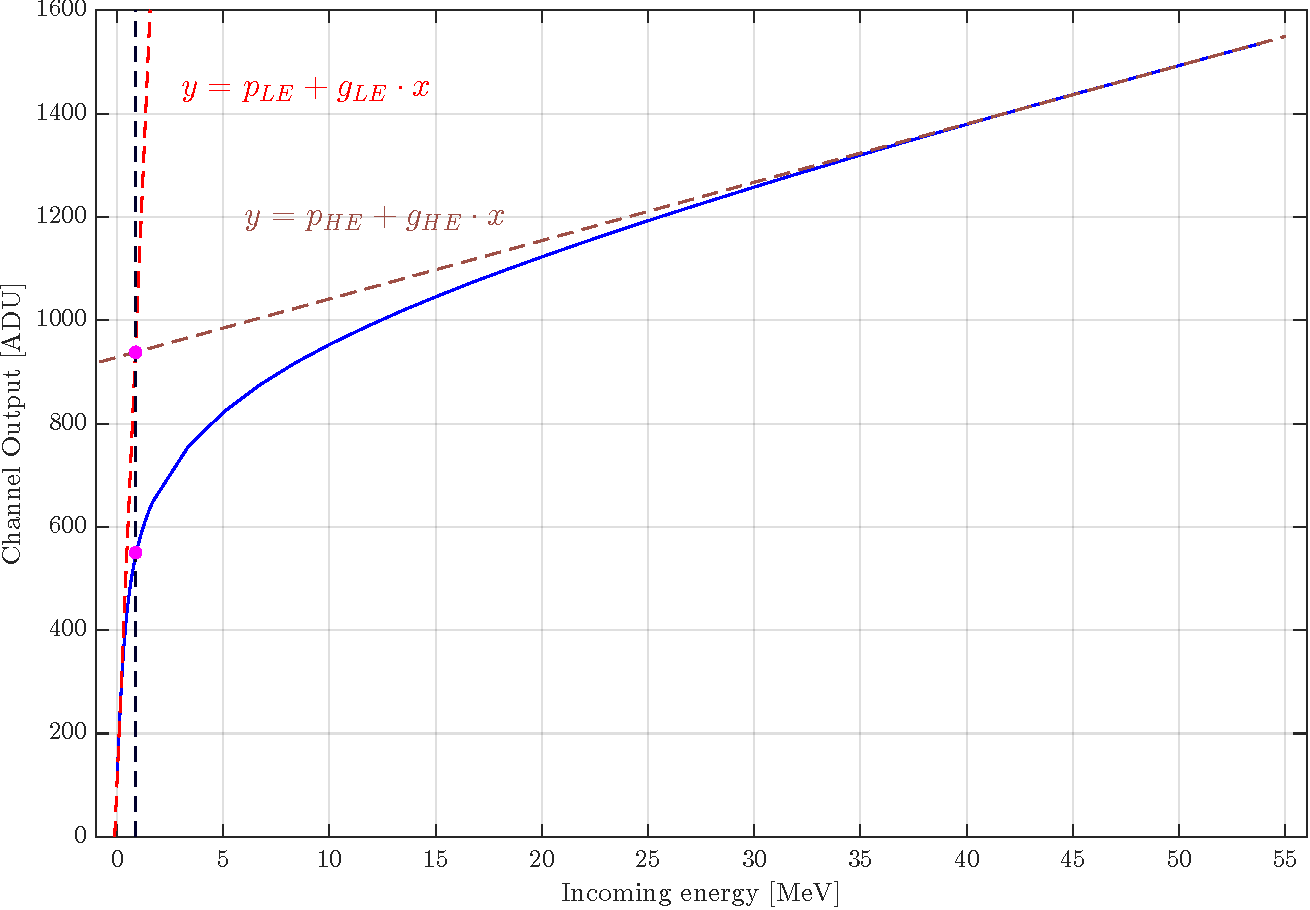
\includegraphics[height=0.42\textheight]{images/temperature_effects/fdt_calcolo_kink.pdf}
        \end{center}
        \vspace{0.05cm}

        \column{0.475\textwidth}
            \textbf{Low and high energy regions gain trend}\\
            \vspace{0.2cm}
            \texttt{CSAVrefGM} = \SI{530}{\milli\volt} @ \SI{-40}{\celsius} $\rightarrow$ low energy gain $\downarrow$
            \vspace{-0.2cm}
            \begin{center}
                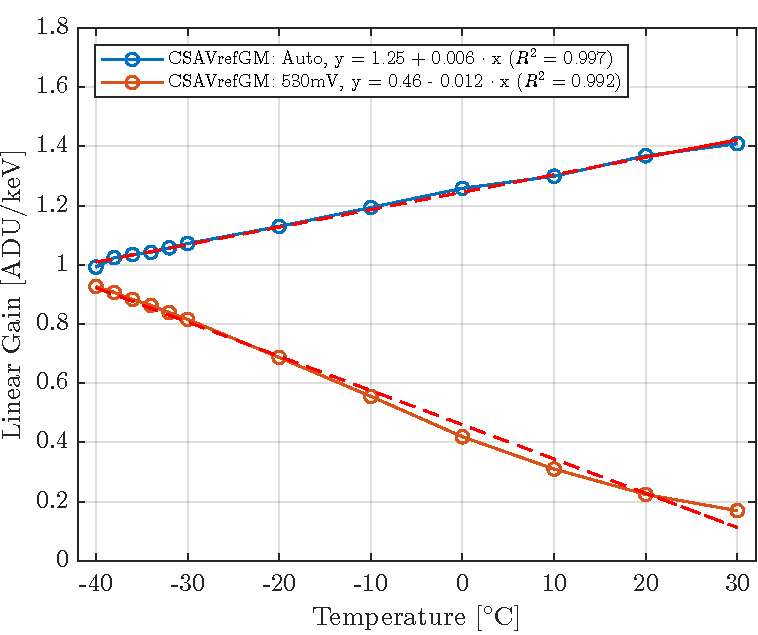
\includegraphics[height=0.32\textheight]{images/temperature_effects/low_energy_gain_auto_530mV.pdf}
                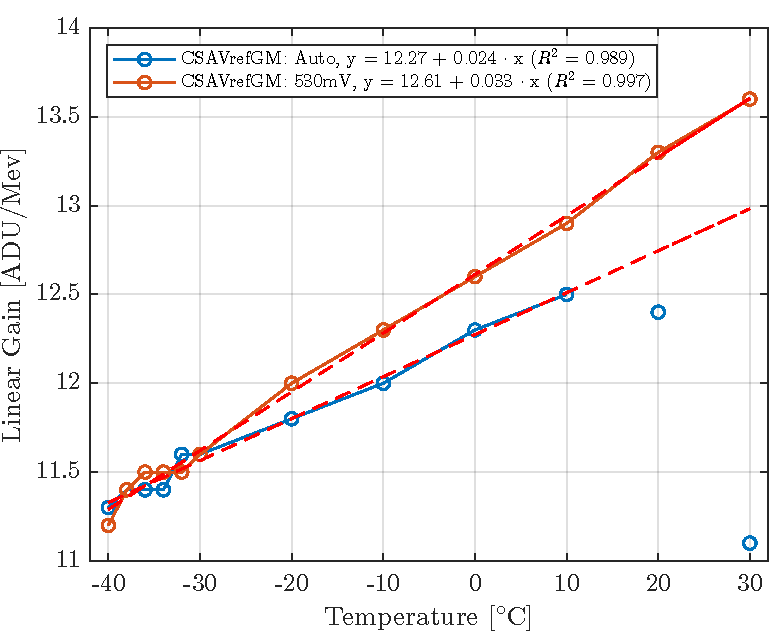
\includegraphics[height=0.32\textheight]{images/temperature_effects/high_energy_gain_auto_530mV.pdf}
            \end{center}

            \textbf{Kink trend as function of temperature}
            \begin{columns}
                \settowidth{\leftmargini}{\usebeamertemplate{itemize item}}
                \addtolength{\leftmargini}{\labelsep}
                \column{0.4\textwidth}
                    \vskip0.1cm
                    \centering
                    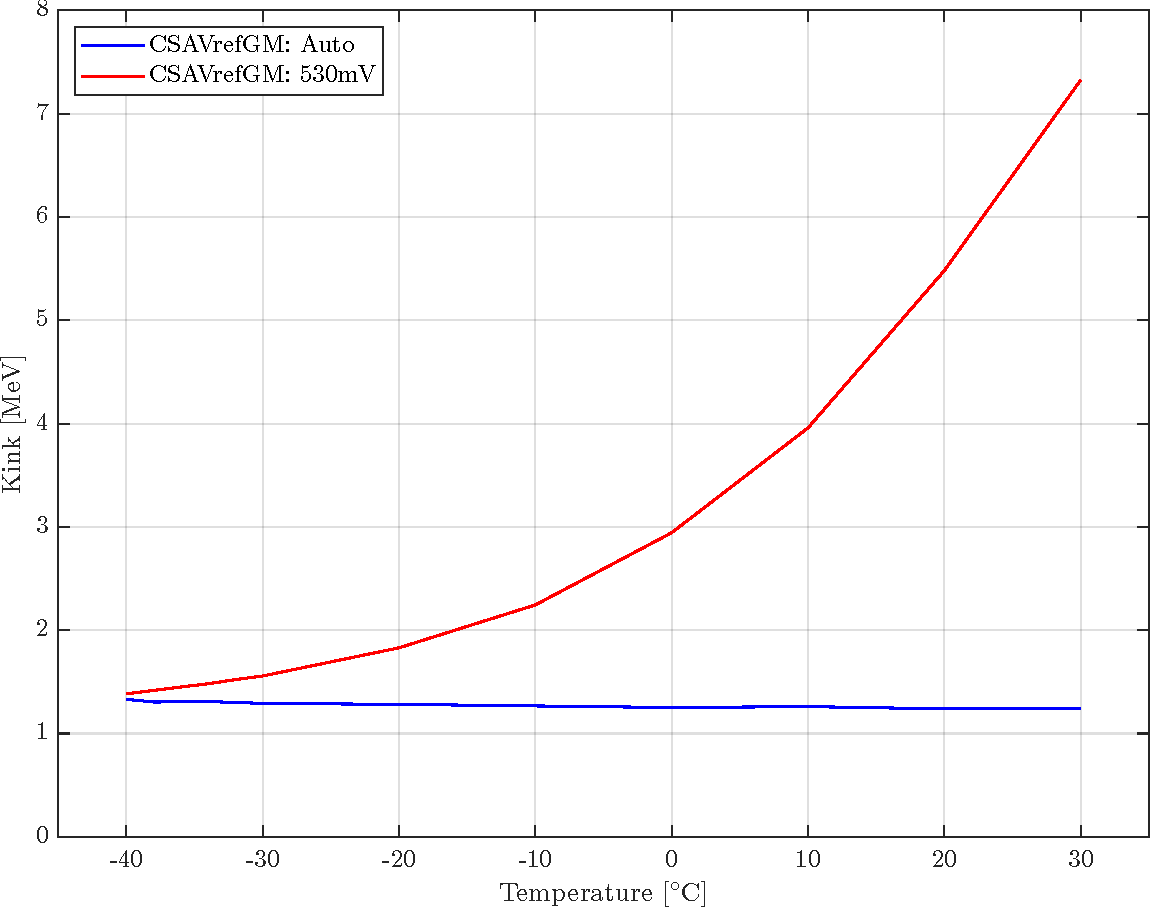
\includegraphics[width=1.15\textwidth]{images/temperature_effects/plot_pedestal_gain_auto_530mV.pdf}
                \column{0.5\textwidth}
                    \raggedleft
                    \begin{itemize}
                        \item \SI{6.95}{\percent} variation around \SI{1.28}{\mega\electronvolt} mean value with auto regulated \texttt{CSAVrefGM} voltage \greencheck
                        \item \SI{429}{\percent} variation with \texttt{CSAVrefGM} voltage\\ fixed to \SI{530}{\milli\volt} \redcross
                    \end{itemize}
            \end{columns}
            \vspace{0.5cm}
    \end{columns}
\end{frame}


%---------------------------------------------------------------------------------------
%	Si(Li) tracker flight components validation
%---------------------------------------------------------------------------------------

\begin{frame}{Si(Li) tracker flight components}
    \fontsize{8.5pt}{1}\selectfont
    \begin{columns}
        \column{0.55\textwidth}
            \begin{tabular}{M{3.8cm} M{3cm}}
                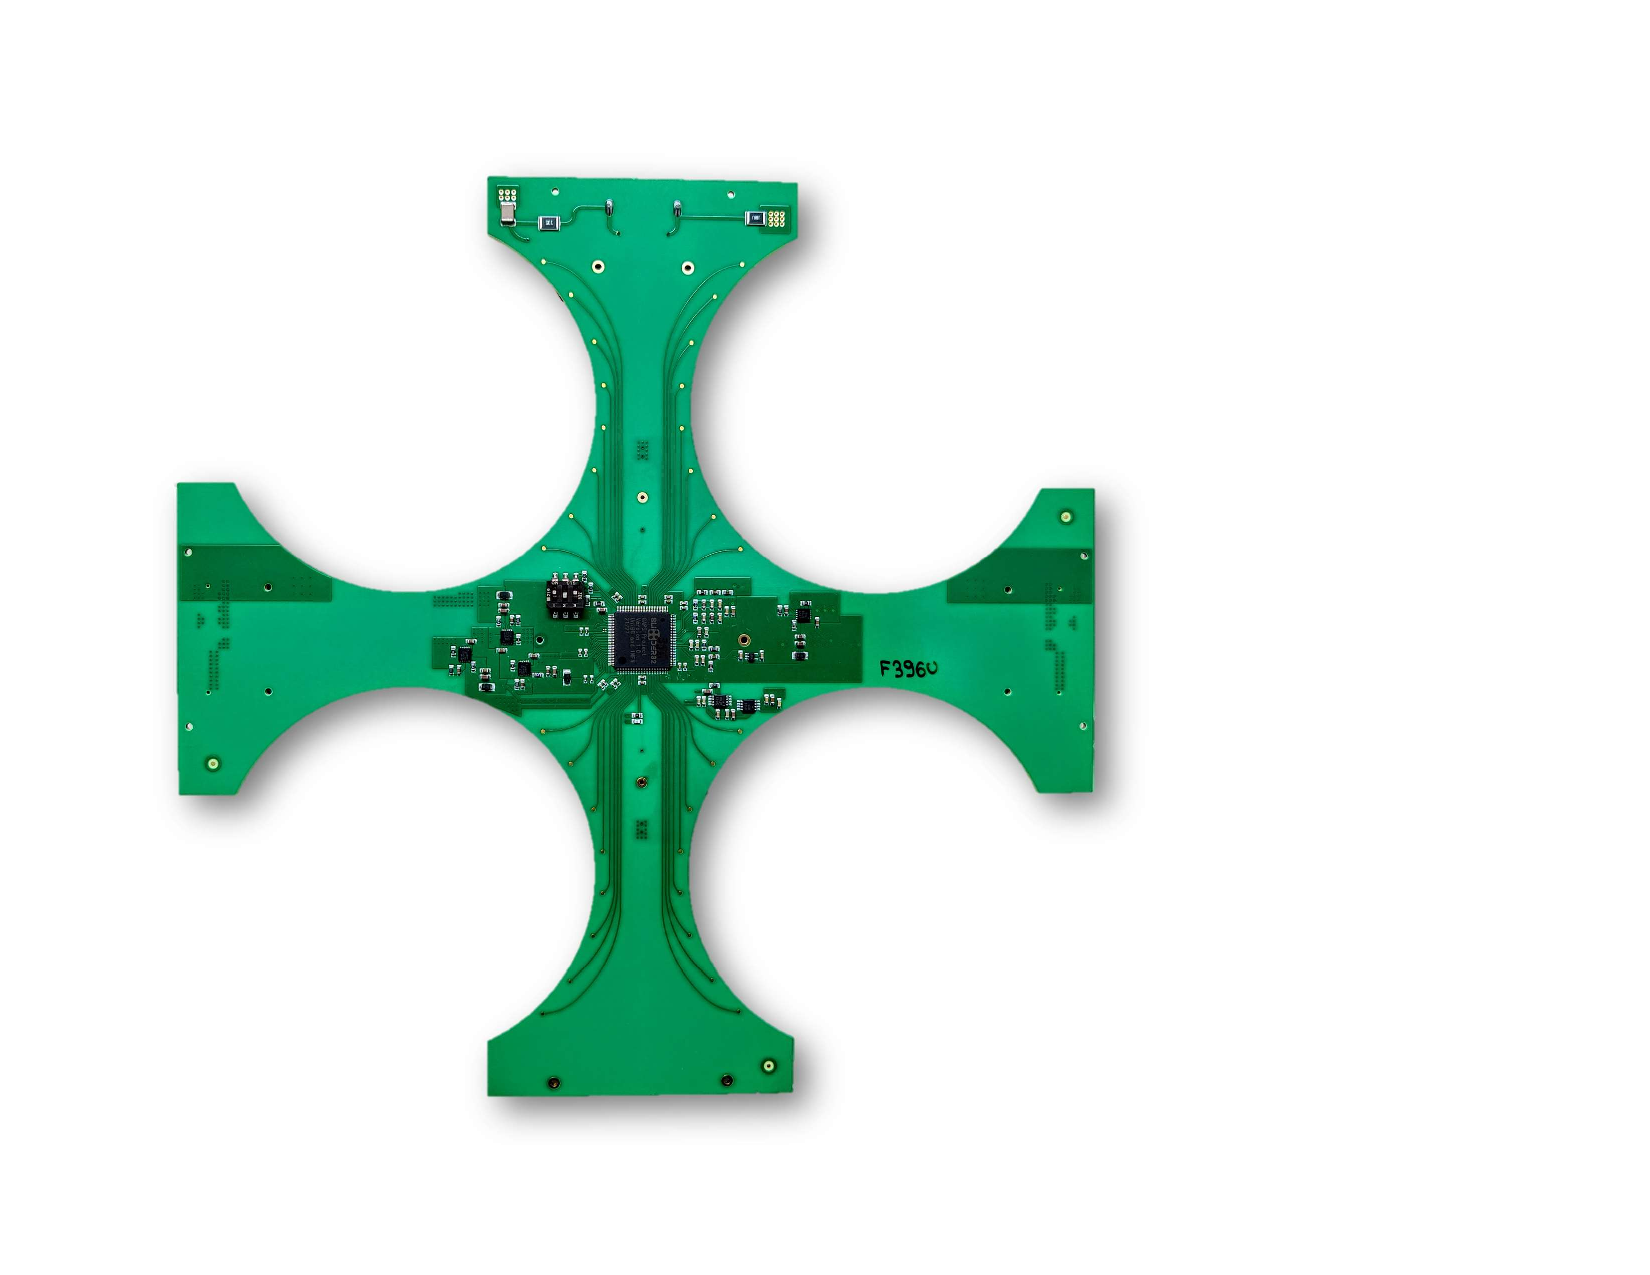
\includegraphics[width=3cm]{images/flight_components_validation/FEB_immagine.pdf} & \shortstack{\textbf{Front-End Board}\vspace{0.2cm} \\ 300 tested} \\\vspace{0.5cm}
                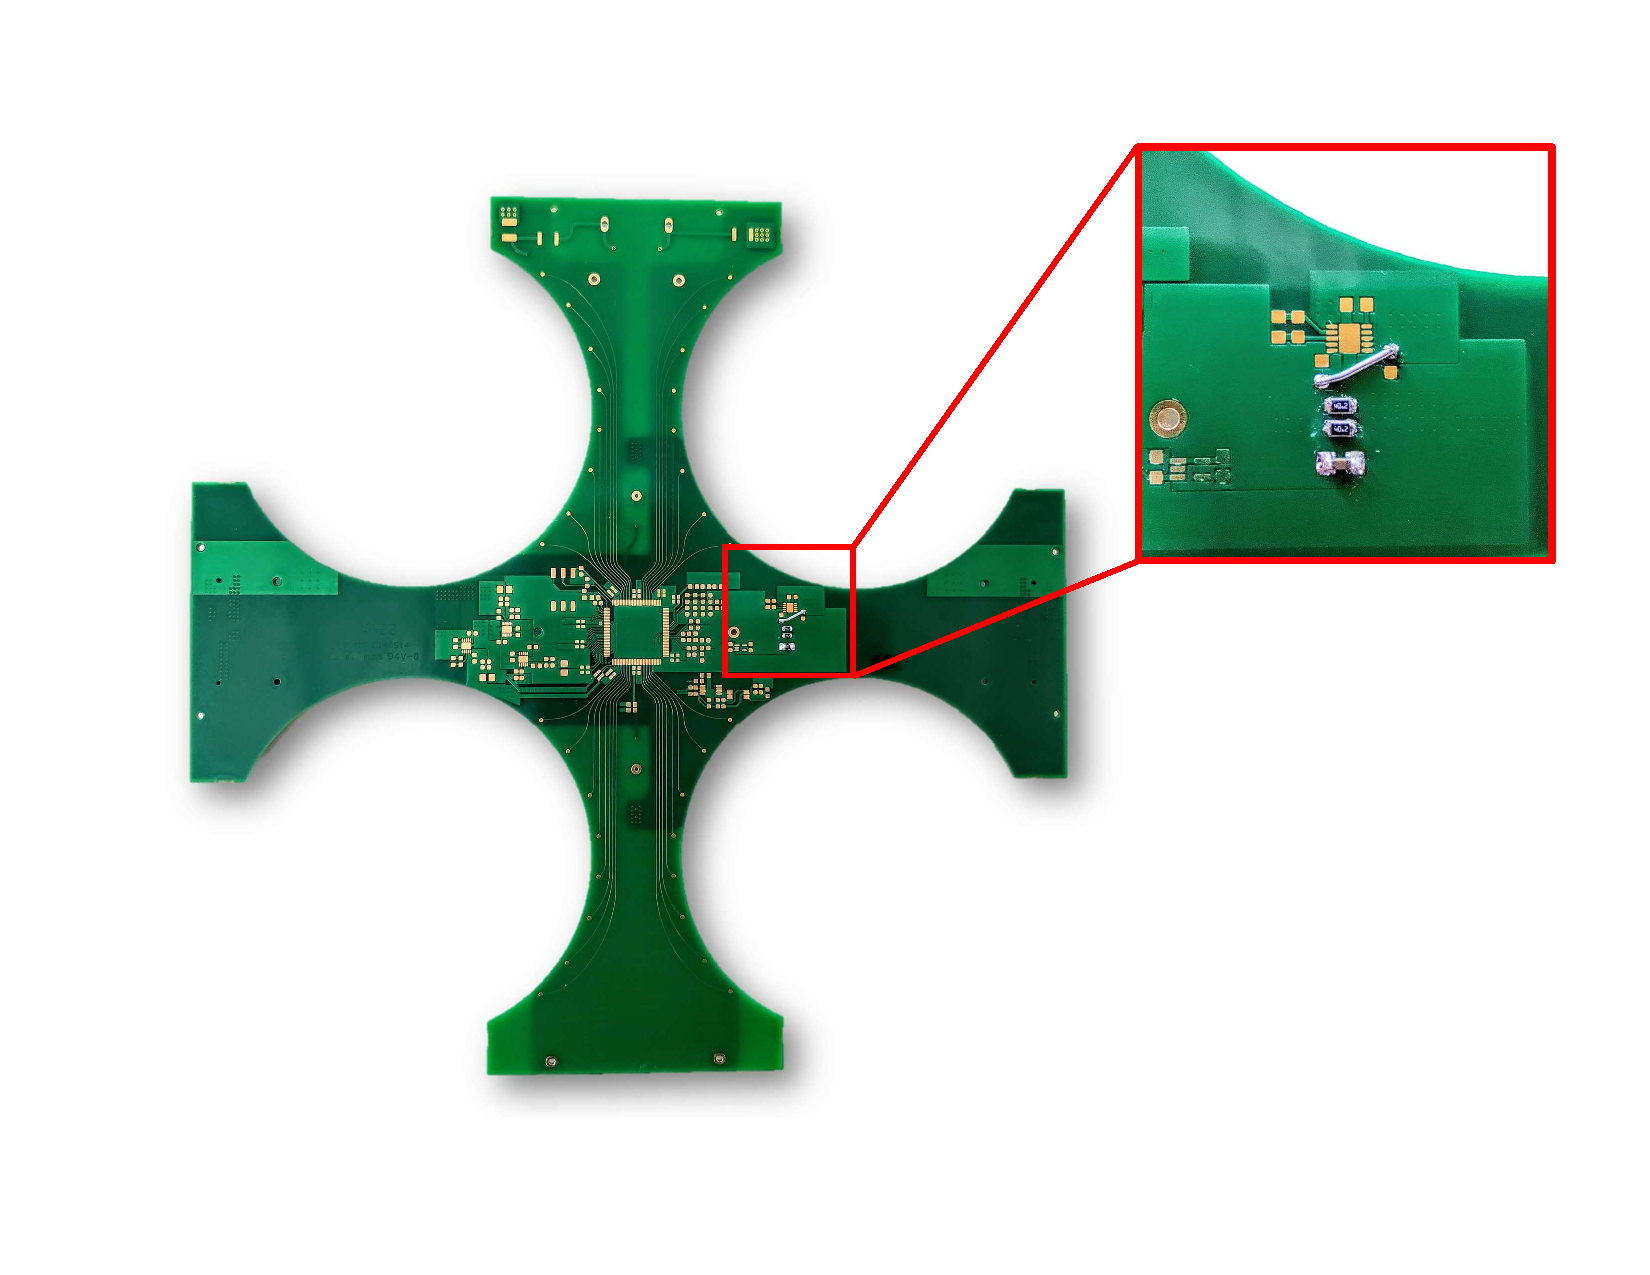
\includegraphics[width=3.8cm]{images/flight_components_validation/dummy_image.pdf} & \shortstack{\textbf{Dummy-1}\\ \textbf{Front-End Board}\vspace{0.2cm} \\ 70 assembled and tested}
            \end{tabular}
        
        \column{0.45\textwidth}
            \begin{tabular}{M{3cm} M{2.5cm}}
                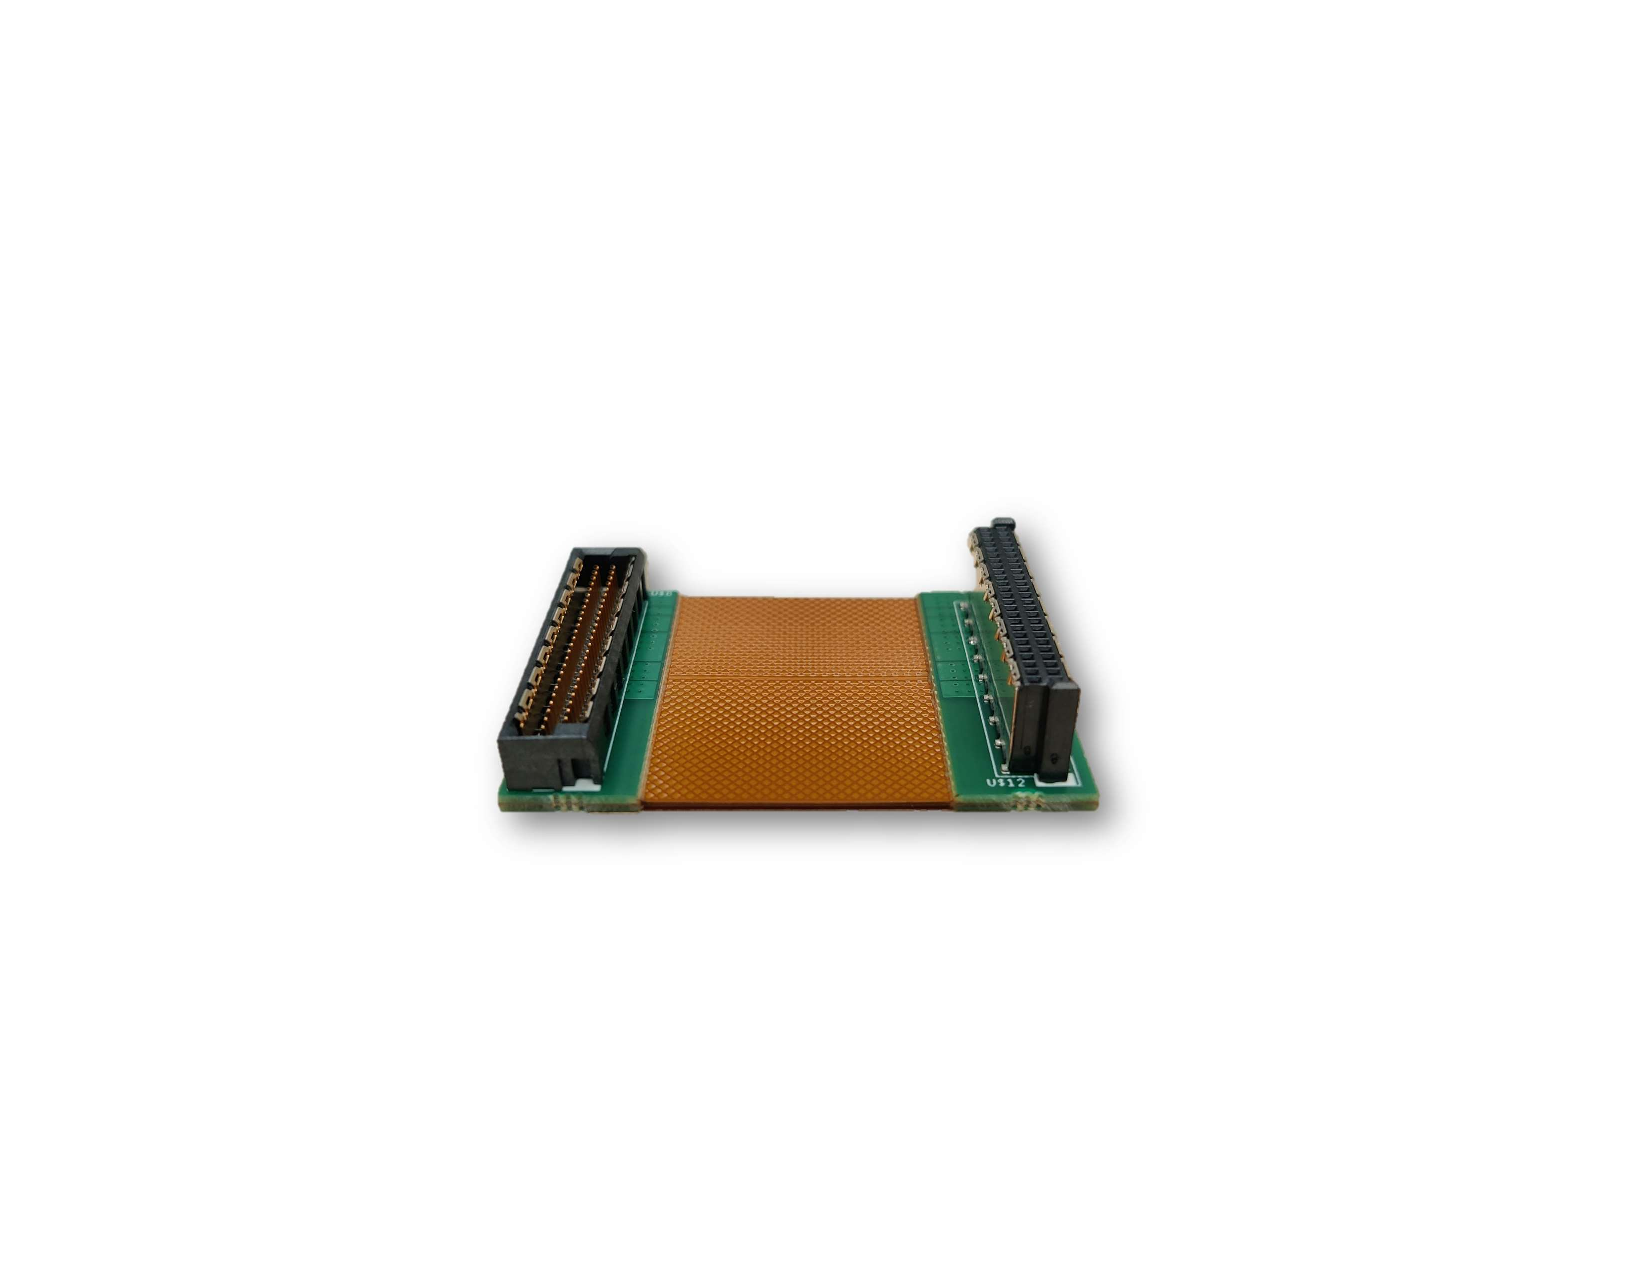
\includegraphics[width=3cm]{images/flight_components_validation/flex_rigid_pic.pdf} & \shortstack{\textbf{Flex-rigid board}\vspace{0.2cm} \\ 300 tested} \\\vspace{0.5cm}
                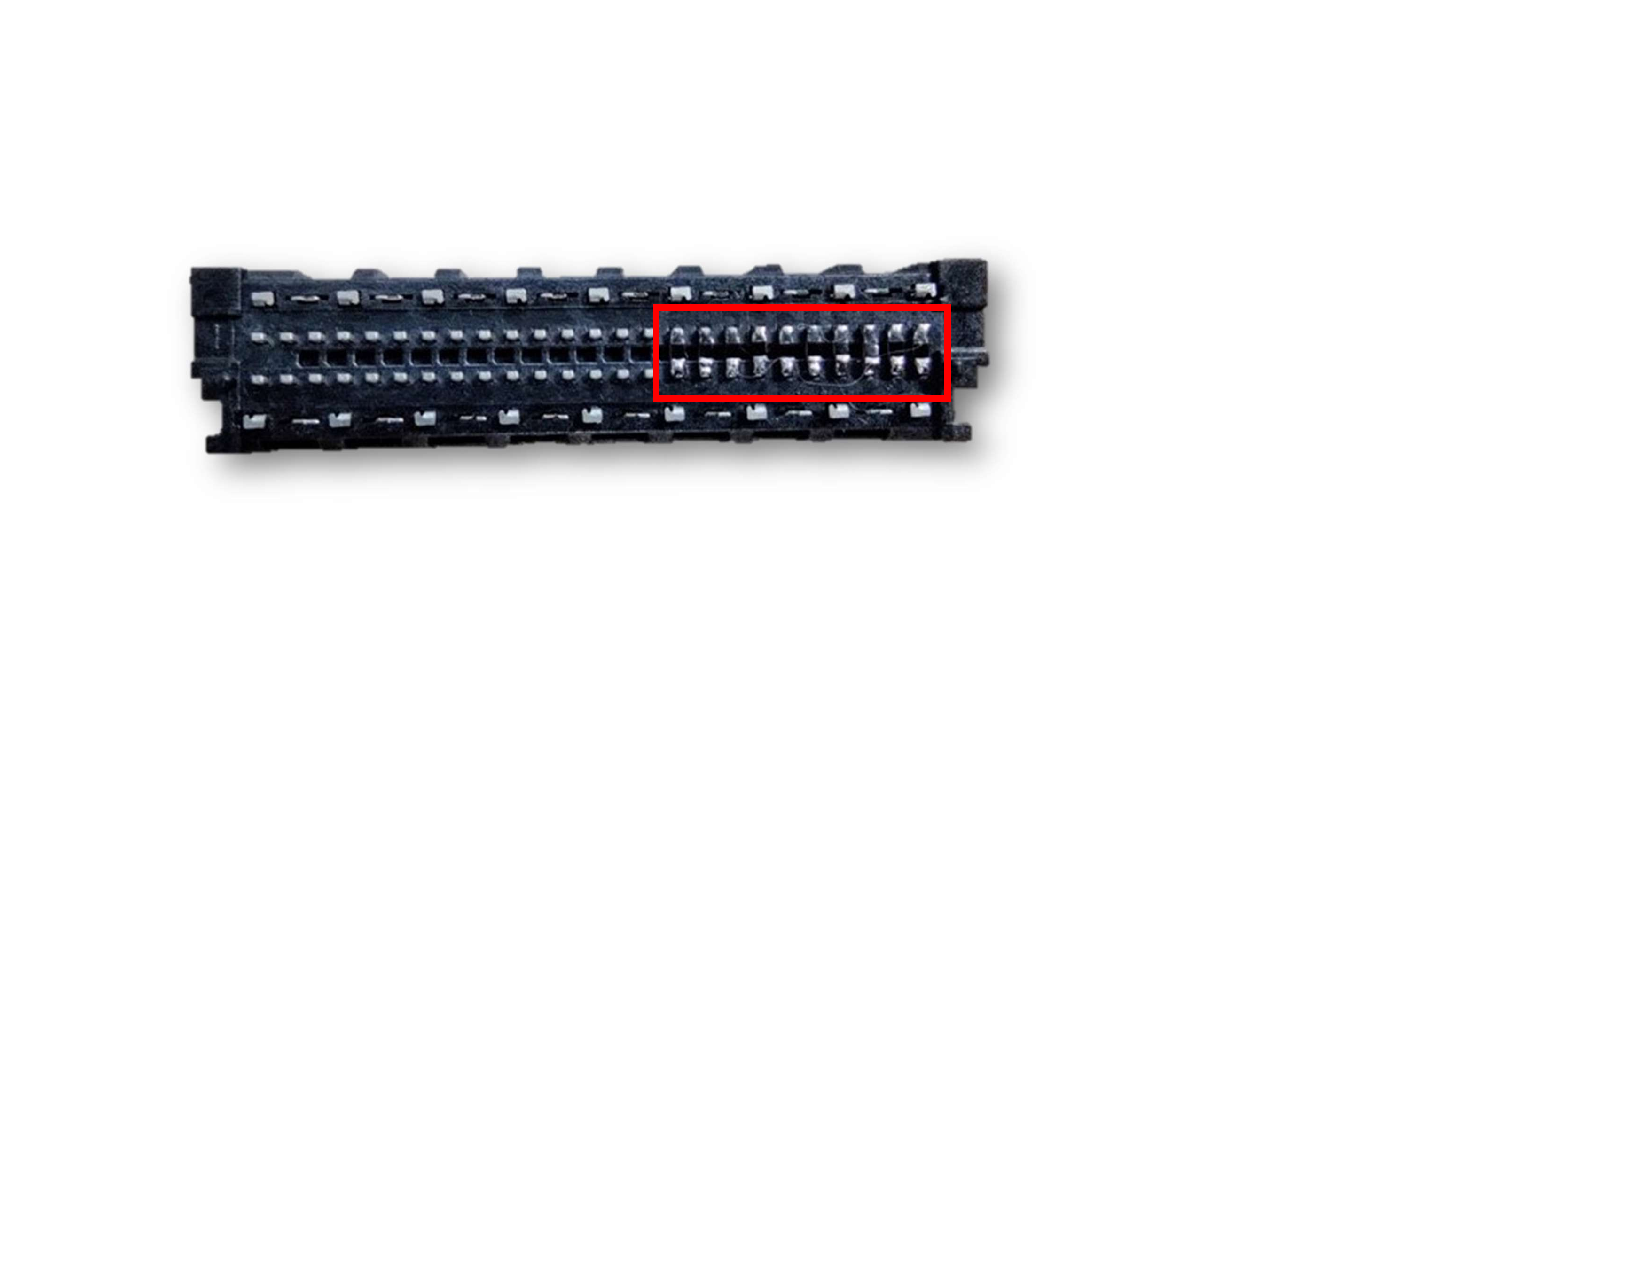
\includegraphics[width=3cm]{images/flight_components_validation/term_conn.pdf} & \shortstack{\textbf{Connector for}\\ \textbf{termination}\vspace{0.2cm} \\ 300 tested} \\\vspace{0.5cm}
                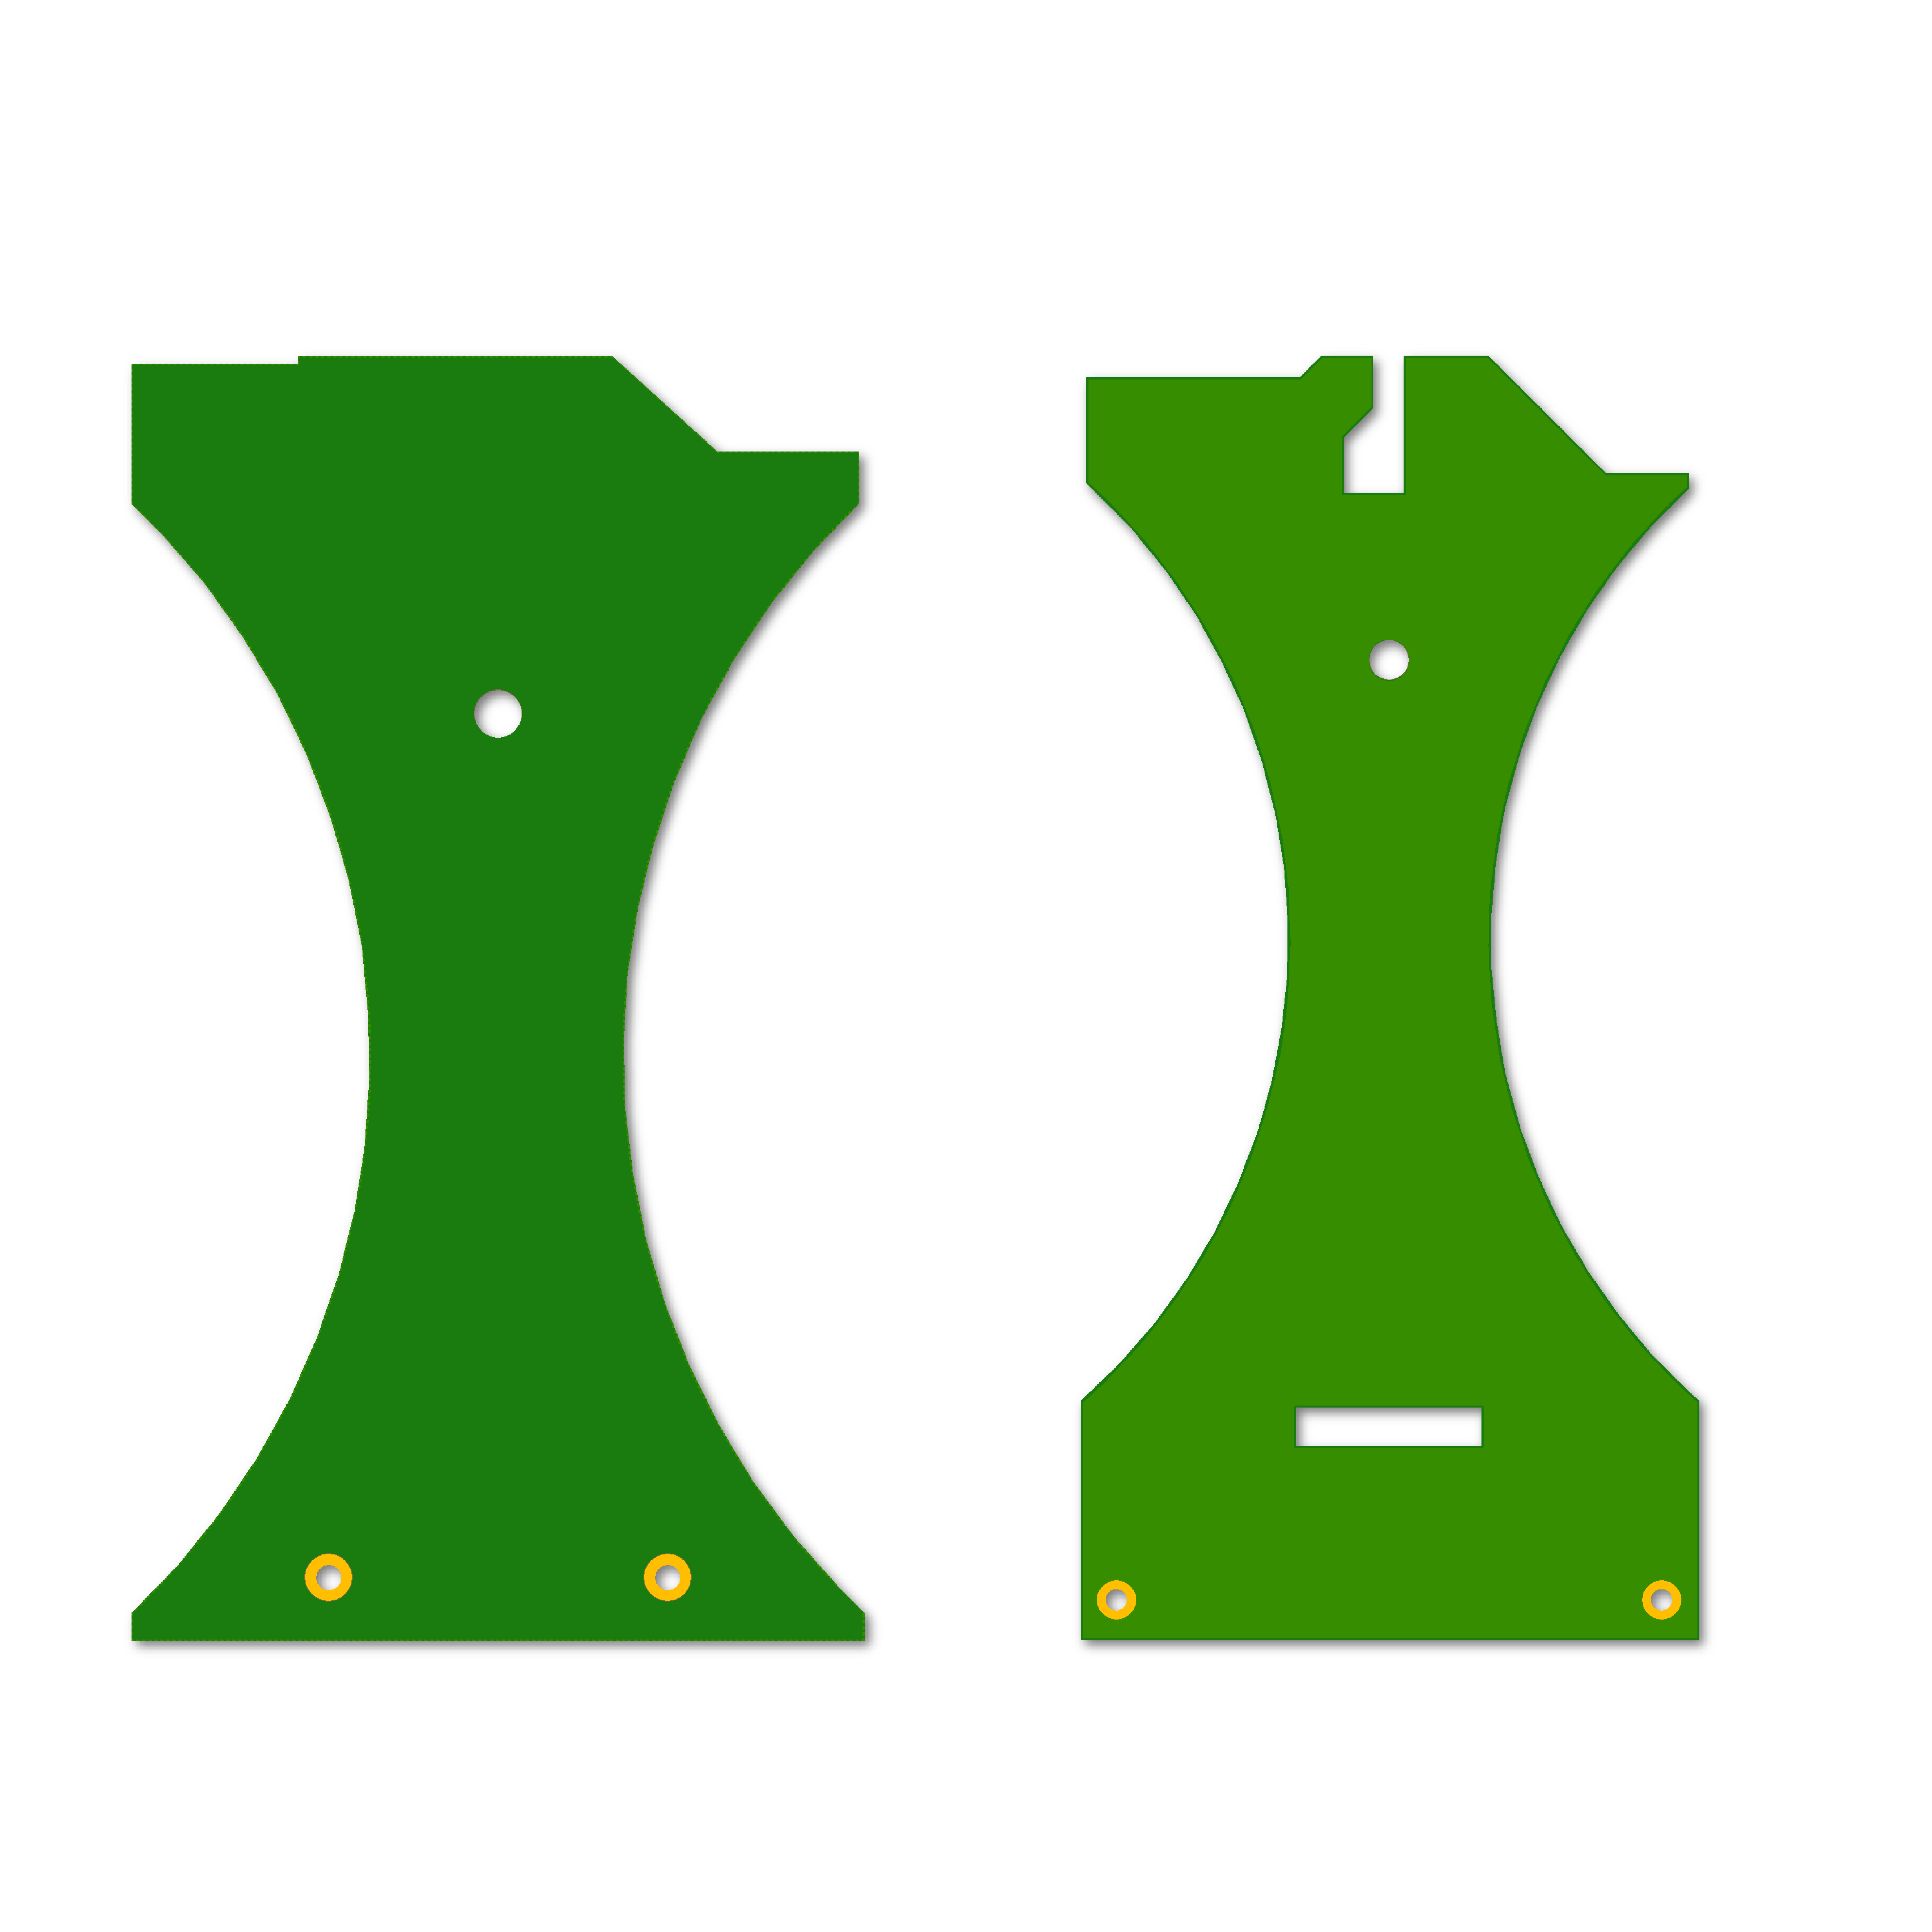
\includegraphics[width=3cm]{images/flight_components_validation/shieldsPDFtwo.pdf} & \shortstack{\textbf{Front-end board}\\ \textbf{shields}\vspace{0.2cm} \\ 300 tested}
            \end{tabular}     
    \end{columns}
\end{frame}


%---------------------------------------------------------------------------------------
%	Si(Li) tracker flight components validation
%---------------------------------------------------------------------------------------

\begin{frame}{Si(Li) tracker flight components validation}
    \fontsize{8.5pt}{1}\selectfont
    \begin{columns}
        \column{0.52\textwidth}
        \textbf{\large \textcolor{ForestGreen}{Validation procedure}}\\
        \vspace{0.15cm}
        Each item has been subjected to a validation procedure that included:
        \begin{itemize}
            \item \textbf{\textcolor{Red}{Thermal cycle}} if not already performed by the manufacturer
            \item \textbf{\textcolor{Red}{Visual inspection}} to search for defects and missing or bad soldered components
            \item \textbf{\textcolor{Red}{Test}} that depends on the item (communication, bias, resistor soldering, ...)
        \end{itemize}

        \vspace{0.2cm}
        At the end of the test procedure:
        \begin{enumerate}
            \item Test results have been saved in a database
            \item An item report with test results has been generated
            \item The item has been classified as
            \begin{itemize}
                \item \textcolor{LimeGreen}{GOOD}
                \item \textcolor{BurntOrange}{USABLE for testing activity only}
                \item \textcolor{OrangeRed}{UNUSABLE}
            \end{itemize}
        \end{enumerate}

        \vspace{0.2cm}
        GOOD and USABLE items have been shipped to \textit{Columbia University} to be used in the final assembly of the experiment at the \textit{MIT Bates} facility in Middleton, Massachusetts
        
        \column{0.42\textwidth}
            \centering
            \vskip0.1cm
            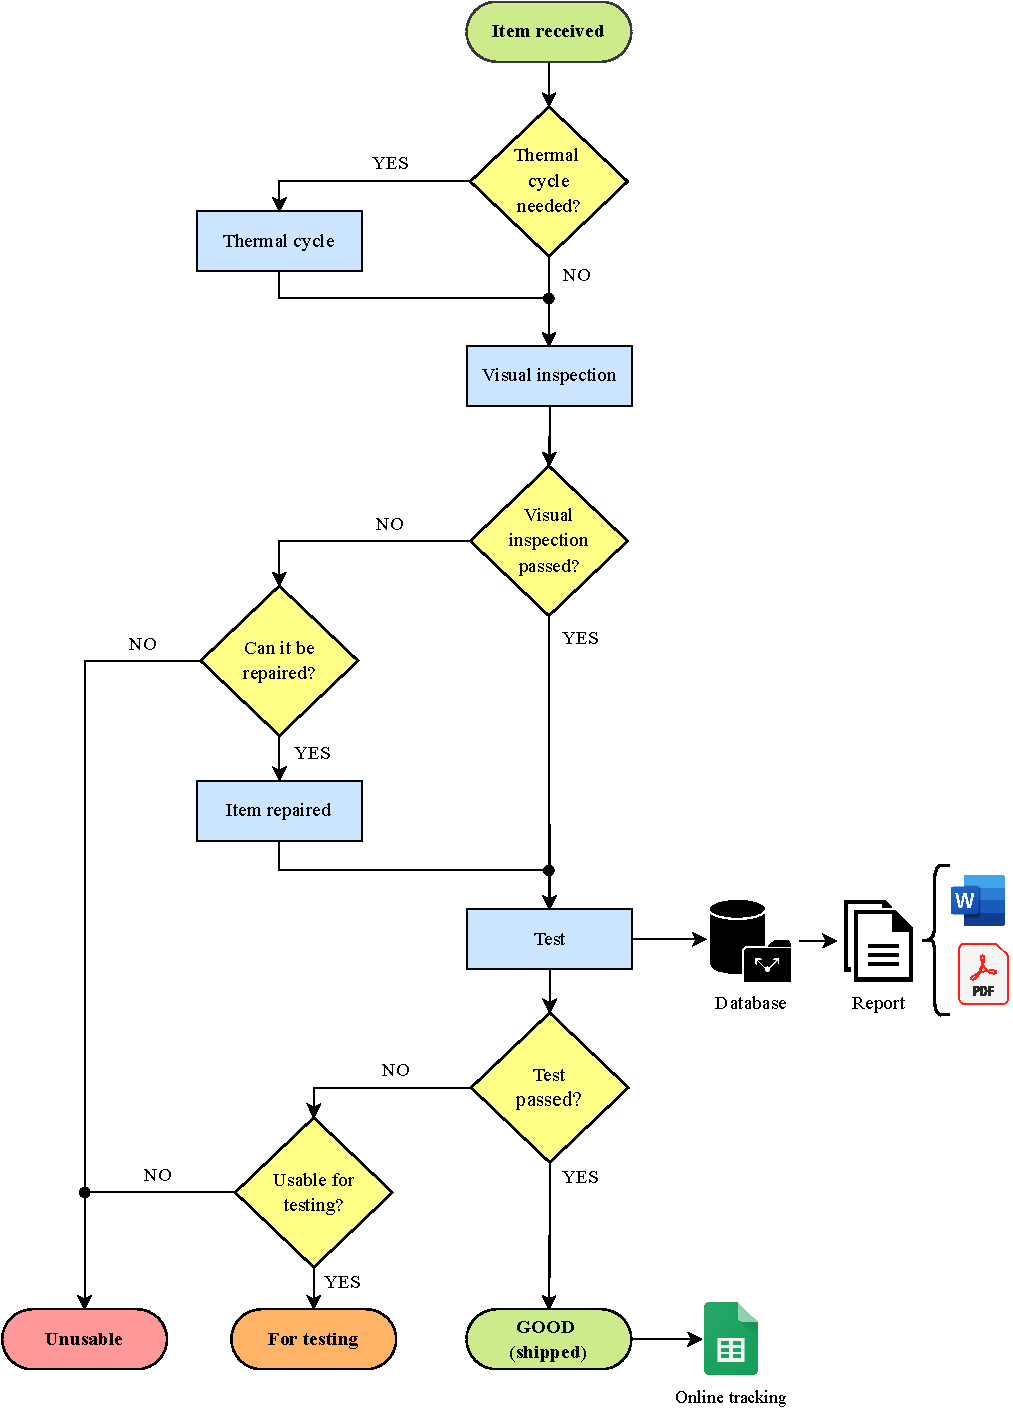
\includegraphics[height=0.85\textheight]{images/flight_components_validation/flight_item_validation_procedure.drawio.pdf}
    \end{columns}
\end{frame}


%---------------------------------------------------------------------------------------
%	Muon detection using an assembled Si(Li) tracker module
%---------------------------------------------------------------------------------------

\begin{frame}{Experimental results from module test}
    \settowidth{\leftmargini}{\usebeamertemplate{itemize item}}
    \addtolength{\leftmargini}{\labelsep}

    \begin{columns}
        \column{0.63\textwidth}

            \fontsize{10pt}{1}\selectfont
            \vskip0.1cm
            \textbf{Si(Li) tracker module test setup} \\
            \vspace{0.05cm}
            
            \fontsize{8.5pt}{1}\selectfont
            \begin{itemize}
                \item Tests performed in a climatic chamber at \SI{-40}{\celsius} and \SI{10}{\percent} humidity
                \item Peaking time \#4 ($\tau_{p} = \SI{0.98}{\micro\second}$)
                \item Self-Trigger mode employed
                \item 1 hour long acquisition
            \end{itemize}
            
            \begin{columns}
                \column{0.6\textwidth}
                    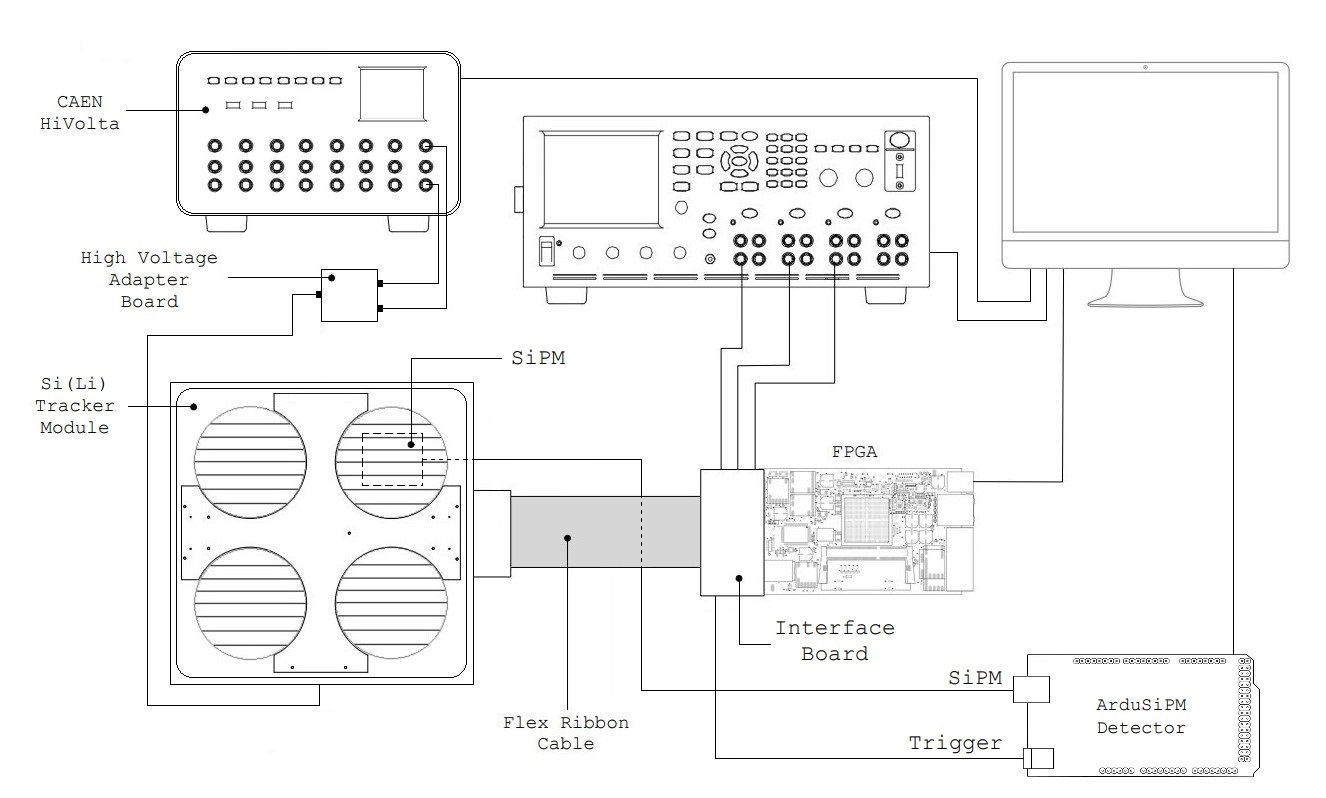
\includegraphics[width=0.99\textwidth]{images/muon_detection/test_setup_MODULE.jpg}
                \column{0.4\textwidth}
                    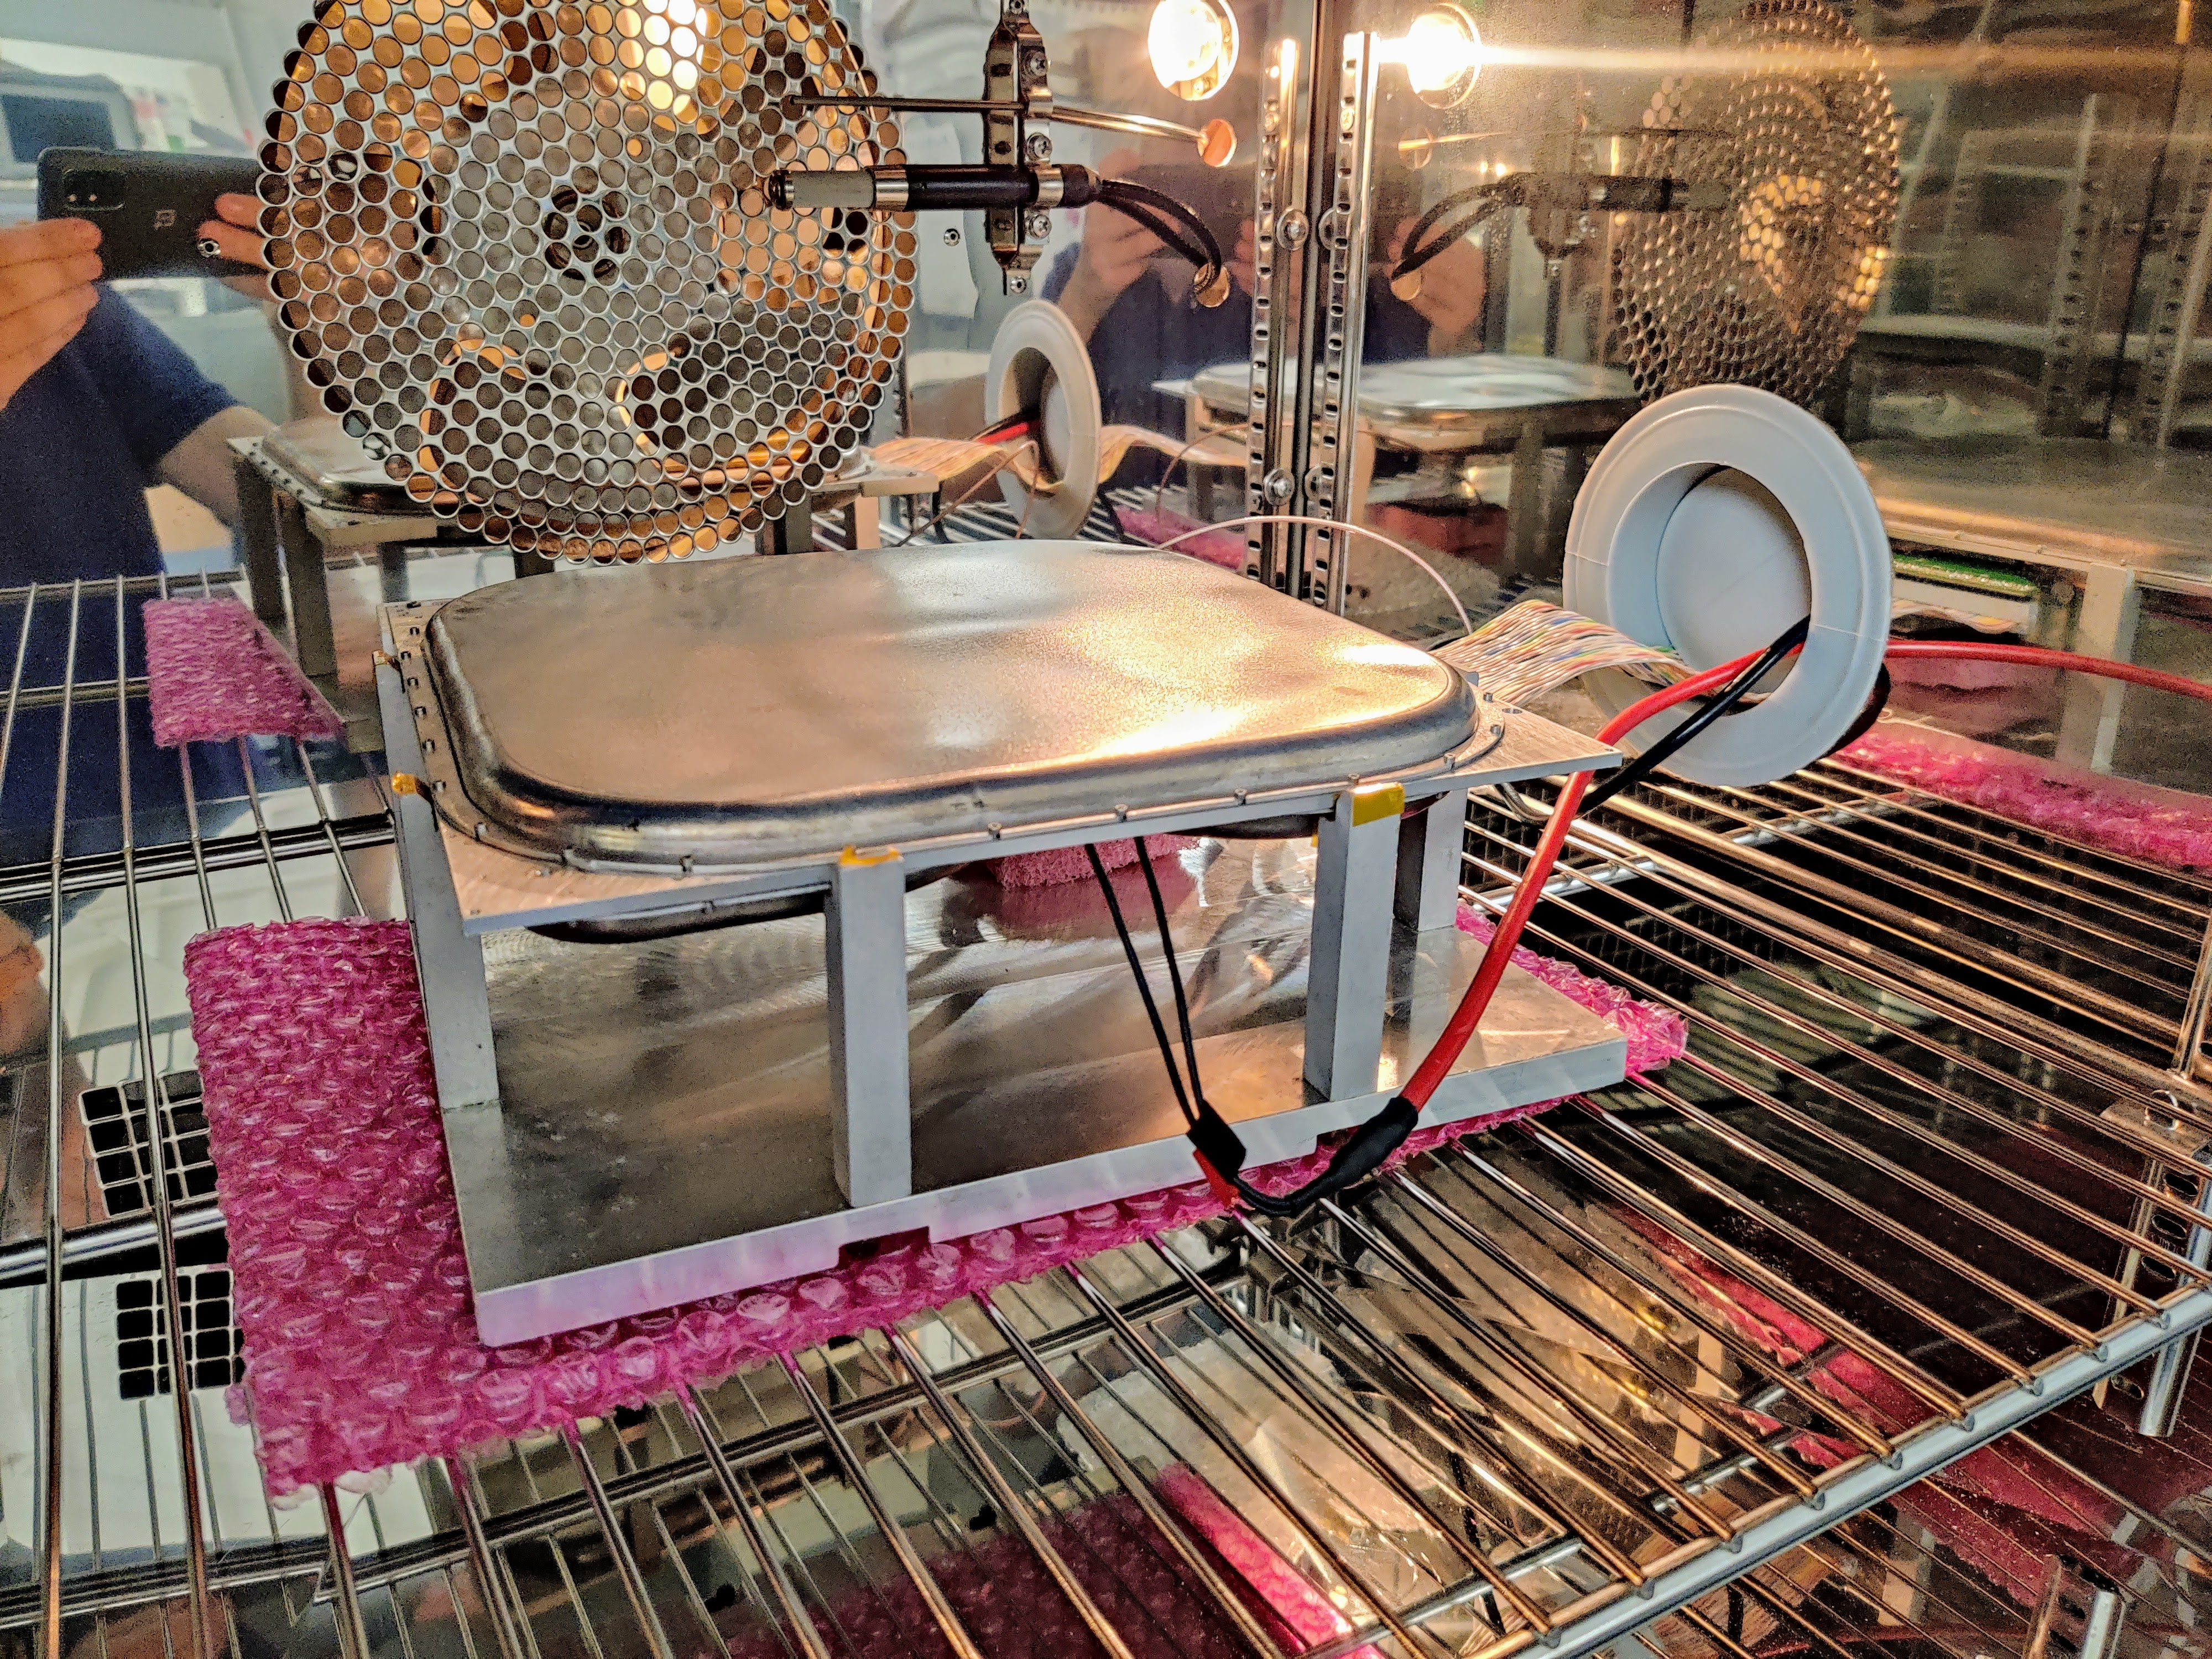
\includegraphics[width=0.9\textwidth]{images/muon_detection/foto_modulo_camera.jpg}
            \end{columns}

            \fontsize{10pt}{1}\selectfont
            \textbf{Results} \\
            \vspace{0.05cm}

            \fontsize{8.5pt}{1}\selectfont
            \begin{itemize}
                \item \SI{59.54}{\kilo\electronvolt} and \SI{26.34}{\kilo\electronvolt} \ce{^{241}Am} $\gamma$ emission peaks detected with visible \textit{Compton Shoulder} \greencheck
                \item Self-Trigger and Zero Suppression modes correctly tested \greencheck
            \end{itemize}

        \column{0.32\textwidth}
            \fontsize{7pt}{1}\selectfont
            \centering
            \textbf{\ce{^{241}Am} source detection} \\
            \vspace{0.1cm}
            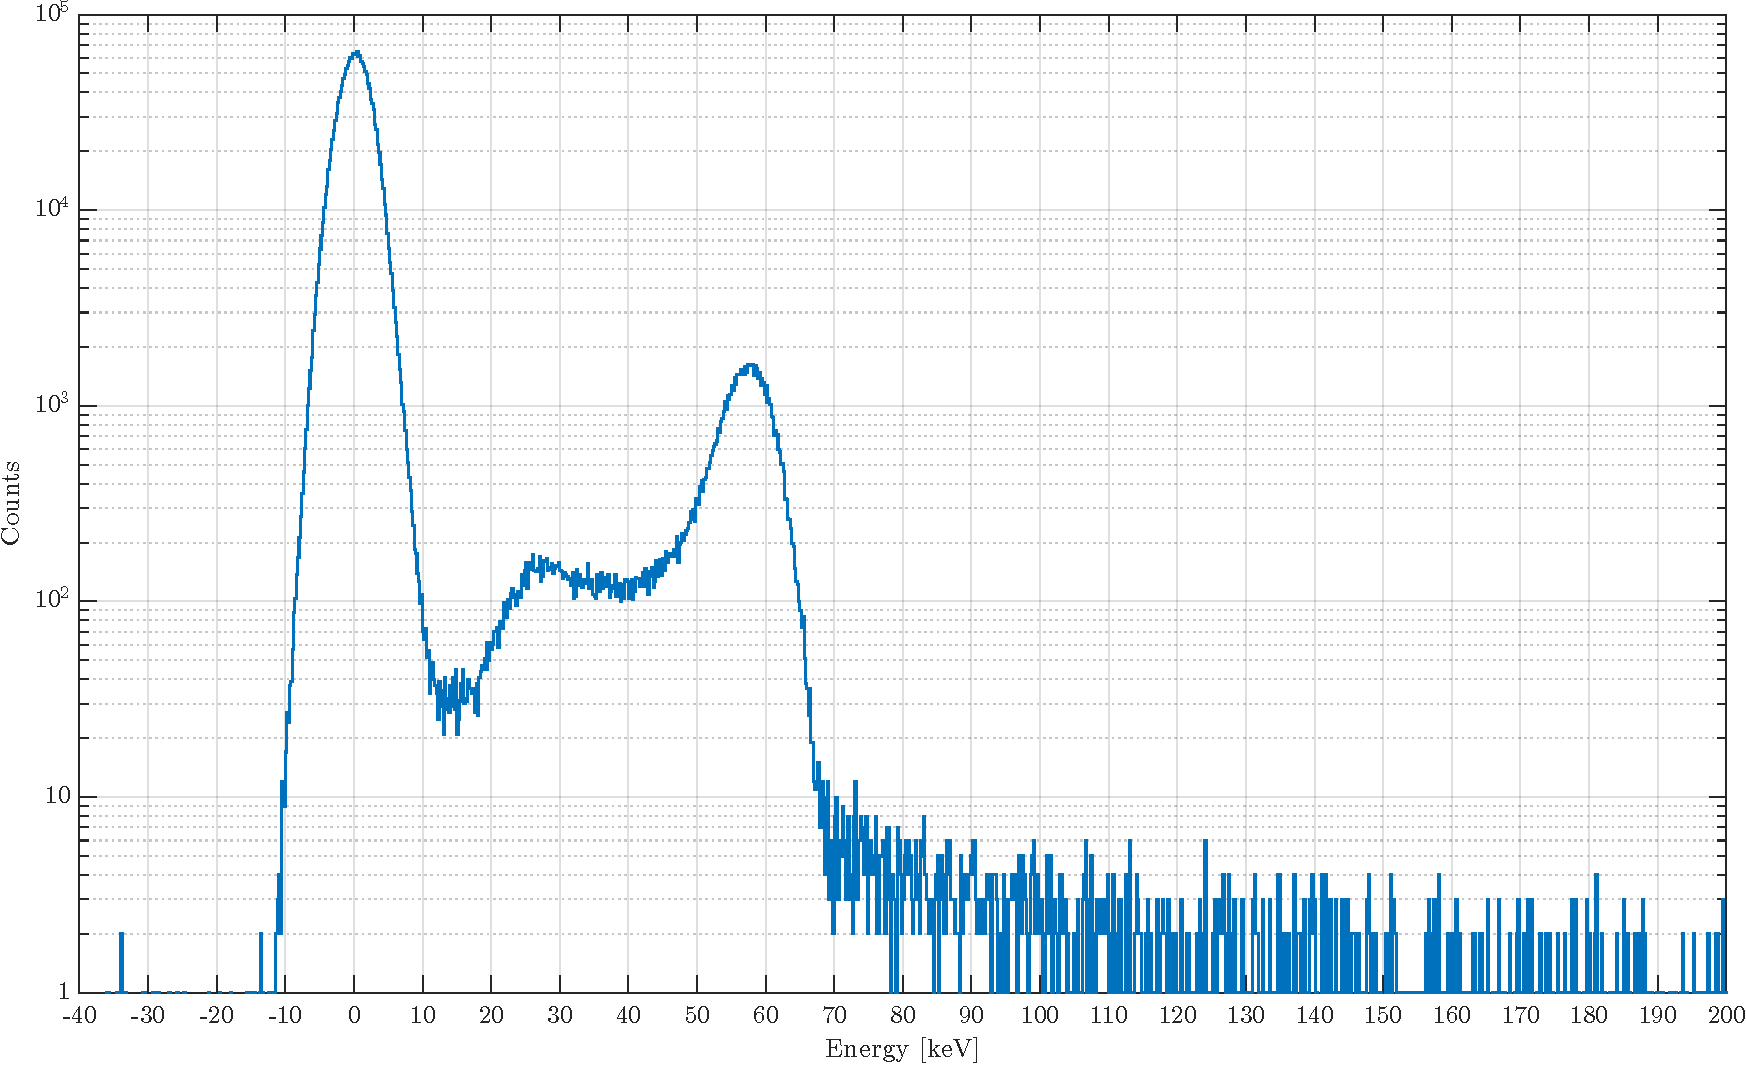
\includegraphics[width=0.99\textwidth]{images/muon_detection/ch4_americio_log.pdf}
            
            \vskip0.15cm
            \textbf{Cosmic muon detection} \\
            \vspace{0.1cm}
            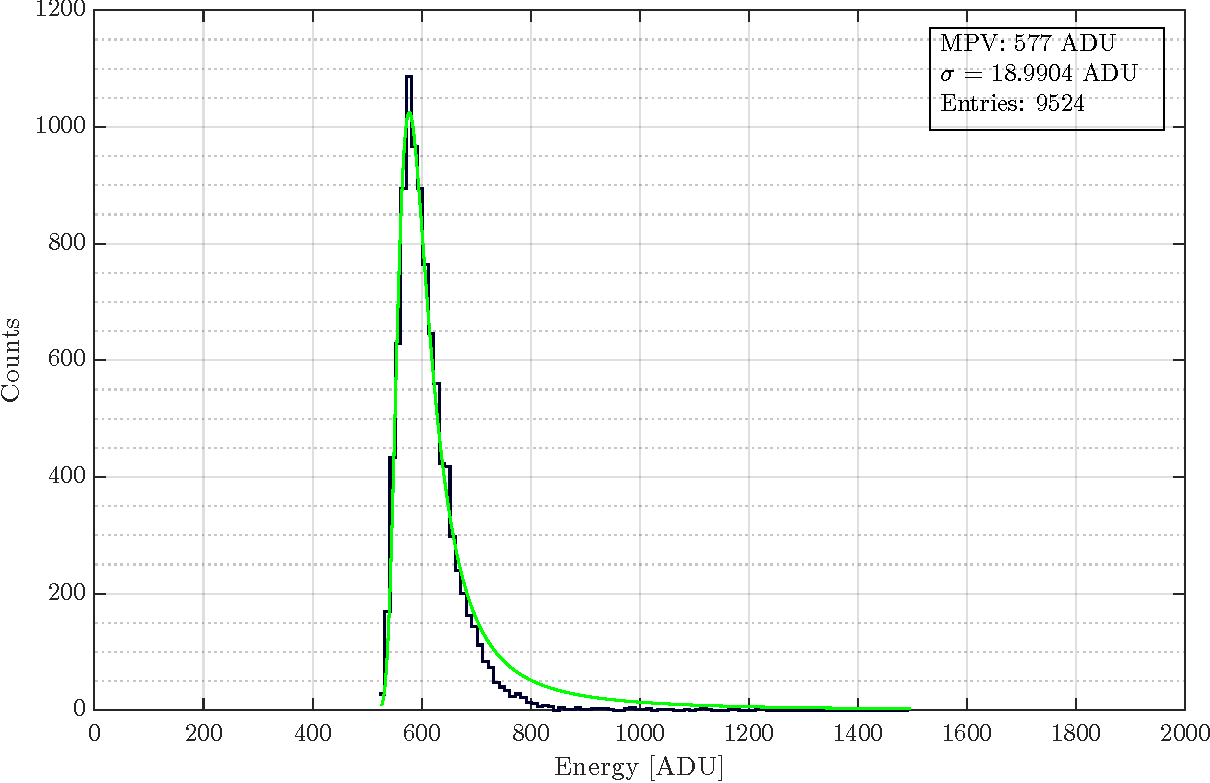
\includegraphics[width=0.99\textwidth]{images/muon_detection/incoming_energy_thr130_ZS_landau.pdf}
    \end{columns}
\end{frame}

\begin{frame}{Cosmic muon detection in\\ \vskip-0.15cm external trigger mode}
    \settowidth{\leftmargini}{\usebeamertemplate{itemize item}}
    \addtolength{\leftmargini}{\labelsep}
    \fontsize{9pt}{1}\selectfont

    \begin{columns}
        \column{0.33\textwidth}
        \begin{itemize}
            \item Scintillator/SiPM assembly placed underneath Si(Li) detector \#2: channels 16 to 23 highlighted in red

            \vskip0.4cm
            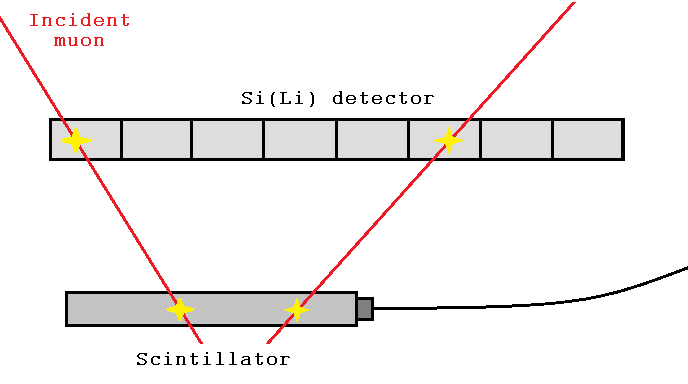
\includegraphics[width=0.9\textwidth]{images/muon_detection/scintillator_sensor_detail.png}

            \vskip0.4cm
            \item \textit{ArduSiPM} device used as an external trigger source
            \item 2 hours acquisition
            \item Global threshold set to \texttt{130}
            \item Trigger hold delay set to \texttt{34} FPGA clocks
            
        \end{itemize}

        \column{0.65\textwidth}
            \vskip-0.2cm
            \begin{figure}[h!]
                \centering
                \begin{tabular}{c c}
                    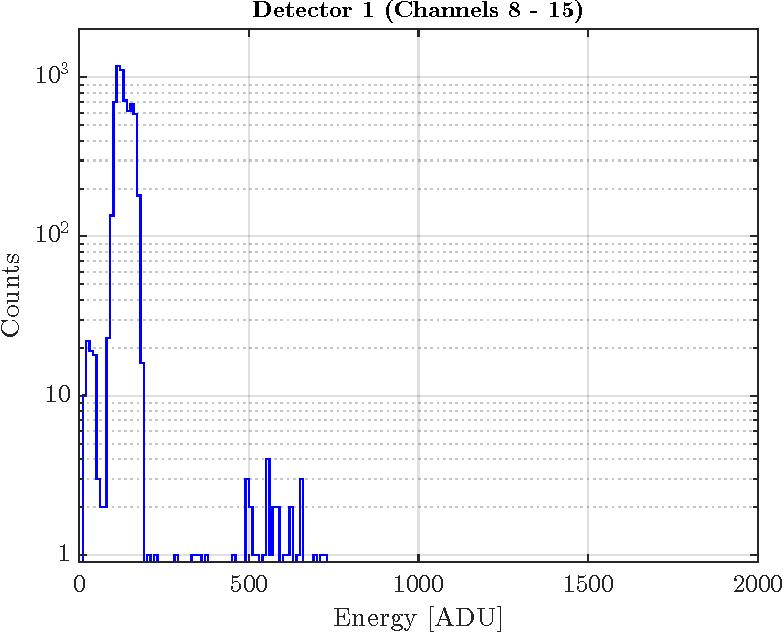
\includegraphics[width=0.44\textwidth]{images/muon_detection/incoming_energy34_2hr_sens2.pdf} & 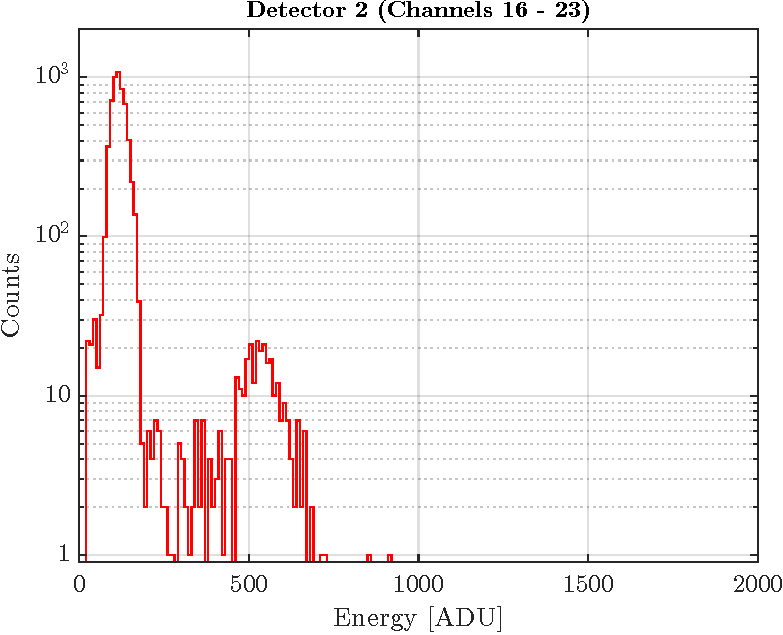
\includegraphics[width=0.44\textwidth]{images/muon_detection/incoming_energy34_2hr_sens3.pdf}\B \\
                    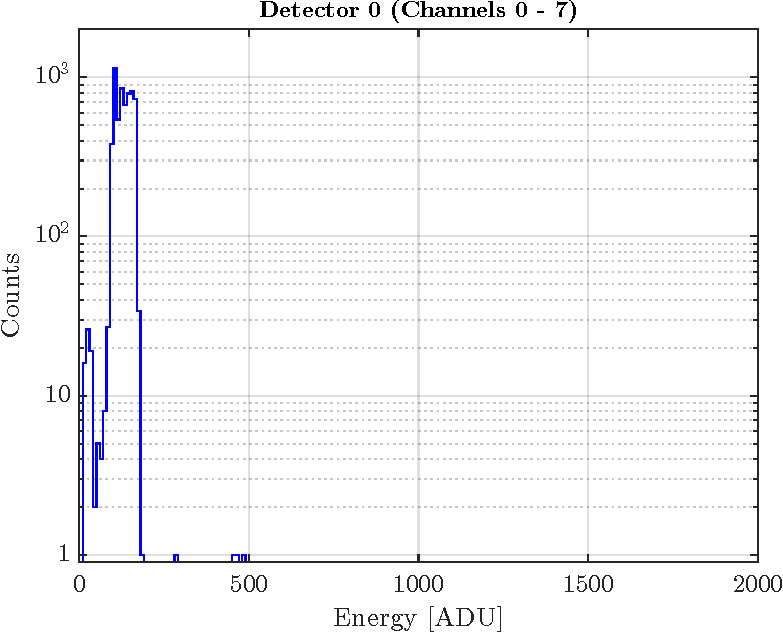
\includegraphics[width=0.44\textwidth]{images/muon_detection/incoming_energy34_2hr_sens1.pdf} & 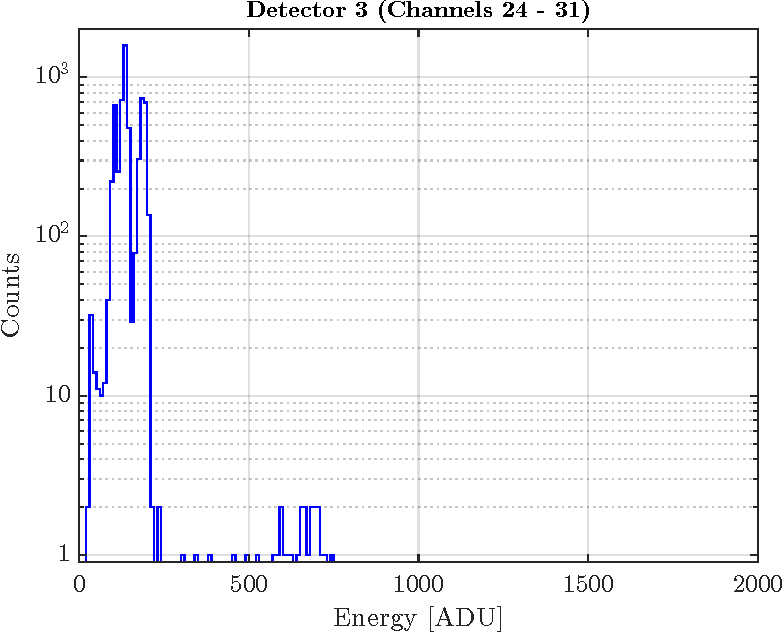
\includegraphics[width=0.44\textwidth]{images/muon_detection/incoming_energy34_2hr_sens4.pdf}
                \end{tabular}
            \end{figure}
        
    \end{columns}
    
\end{frame}

%---------------------------------------------------------------------------------------
%	Conclusions
%---------------------------------------------------------------------------------------

\section{Conclusions}

\begin{frame}{Conclusions}
    txt
\end{frame}


%---------------------------------------------------------------------------------------
%	Backup slides
%---------------------------------------------------------------------------------------

\appendix
\backupbegin

\begin{frame}[plain]{}
    \fontsize{20pt}{1}\selectfont
    \centering
    \vspace{1.5cm}
    \textbf{Backup slides}
\end{frame}

\begin{frame}{Analog readout channel and ADC}
    \fontsize{8.5pt}{1}\selectfont
    \settowidth{\leftmargini}{\usebeamertemplate{itemize item}}
    \addtolength{\leftmargini}{\labelsep}
    \centering
    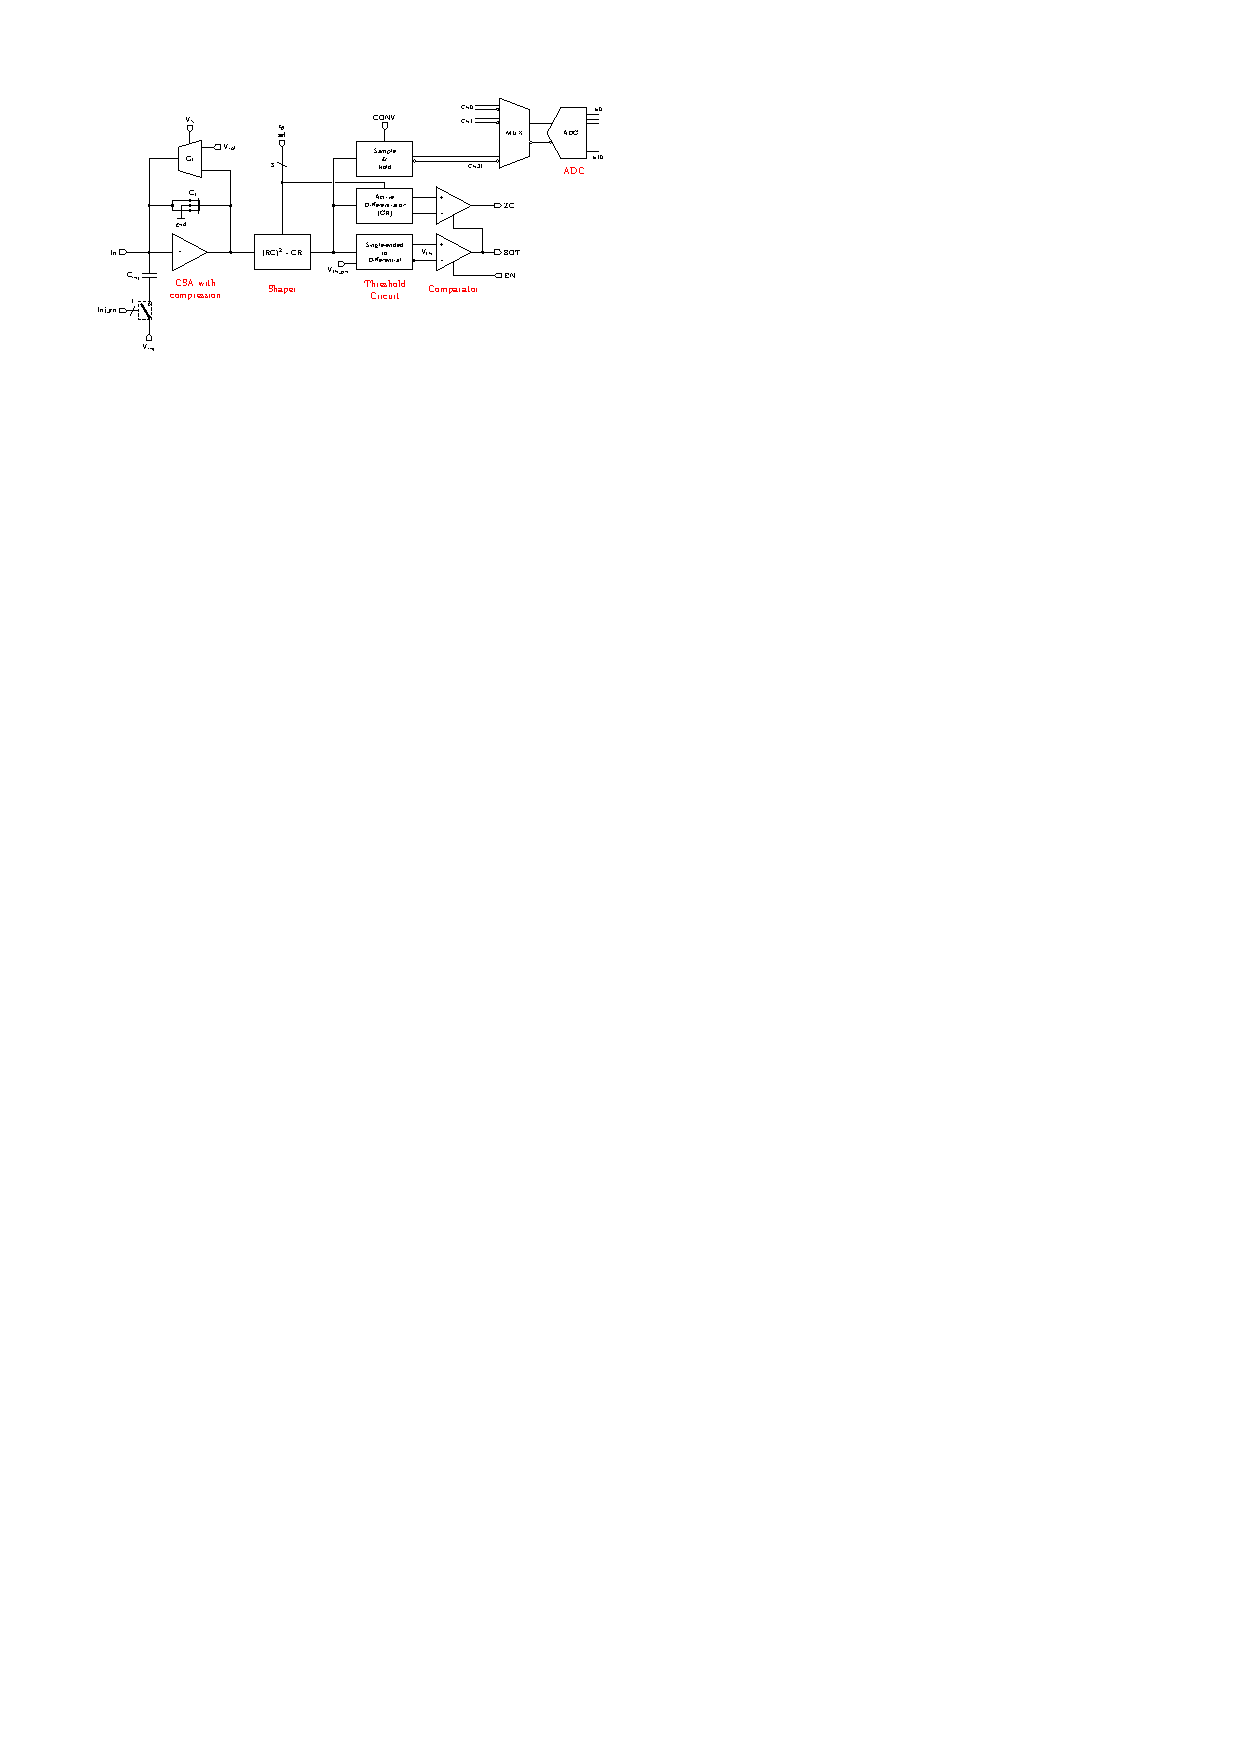
\includegraphics[width=0.68\textwidth]{images/backup_slides/readoutchannelADC.pdf}

    \vskip0.2cm
    
    \begin{columns}[T]
        \column{0.3\textwidth}
            \begin{itemize}
                \item \textbf{Charge Sensitive Amplifier}\\ with dynamic signal compression
                \item \textbf{CR-(RC)$^{2}$ filter}\\ with 8 selectable peaking times (from \SI{250}{\nano\second} to \SI{1.8}{\micro\second})
            \end{itemize}
            
        \column{0.36\textwidth}
            \begin{itemize}
                \item \textbf{SOT comparator}\\ Signal Over Threshold identification
                \item \textbf{Active CR and ZC comparator}\\ Shaper signal peak detection
                \item \textbf{Single-ended to differential S\&H}\\ Shaper signal peak storage
            \end{itemize}
        
        \column{0.25\textwidth}
            \begin{itemize}
                \item \textbf{Injection capacitance $C_{inj}$}\\ Used for calibration
                \item \textbf{11-bit hybrid SAR ADC} \\ One per ASIC with 32:1 multiplexer
            \end{itemize}
    \end{columns}
\end{frame}


\begin{frame}{SLIDER32 ASIC}
   \begin{columns}
    \column{0.6\textwidth}
        \fontsize{10pt}{1}\selectfont
        \textbf{\textcolor{ForestGreen}{SLIDER: SiLI DEtector Readout}}\\
        \vspace{0.3cm}
        \fontsize{9.5pt}{1}\selectfont
        \textbf{\textcolor{Red}{ASIC features}}
        \vspace{0.1cm}
        \begin{itemize}
            \fontsize{9pt}{1}\selectfont
            \setlength\itemsep{0.3em}
            \item \SI{180}{\nano\meter} CMOS technology design
            \item 32 channels per ASIC
            \item -\SI{40}{\celsius} operating temperature
            \item Digital Back End (registers control, SPI, ...)
            \item BGR with 3-bit DAC regulation
            \item 8-bit DAC for global threshold setting
            \item 3-bit DAC for threshold fine trimming
            \item Detector leakage current readout
            \item Temperature sensor readout
            \item low-noise \textbf{Charge Sensitive Amplifier} (CSA) performing dynamic signal compression
            \item unipolar second order semi-Gaussian \textbf{time invariant filter}
            \item single-ended to differential \textbf{Sample \& Hold} (S\&H)
            \item 11-bit \textbf{Analog to Digital Converter} (ADC)
        \end{itemize}
  
    \column{0.35\textwidth}
        \begin{figure}
        \centering
        \vspace{-0.25cm}
        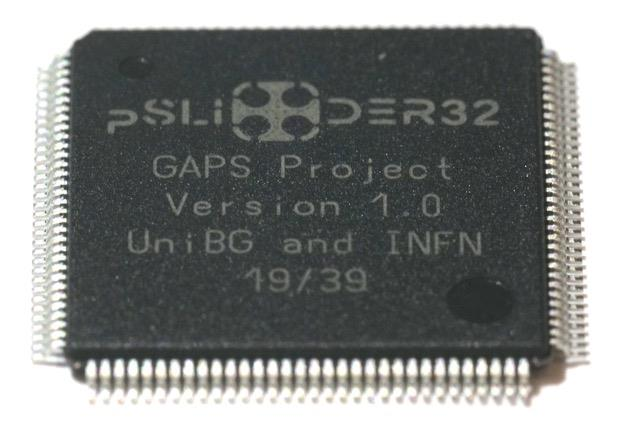
\includegraphics[height=0.2\textheight]{images/backup_slides/SLIDER32_asic_package.jpg}
        \vspace{0.2cm}
        \vskip0.001cm
        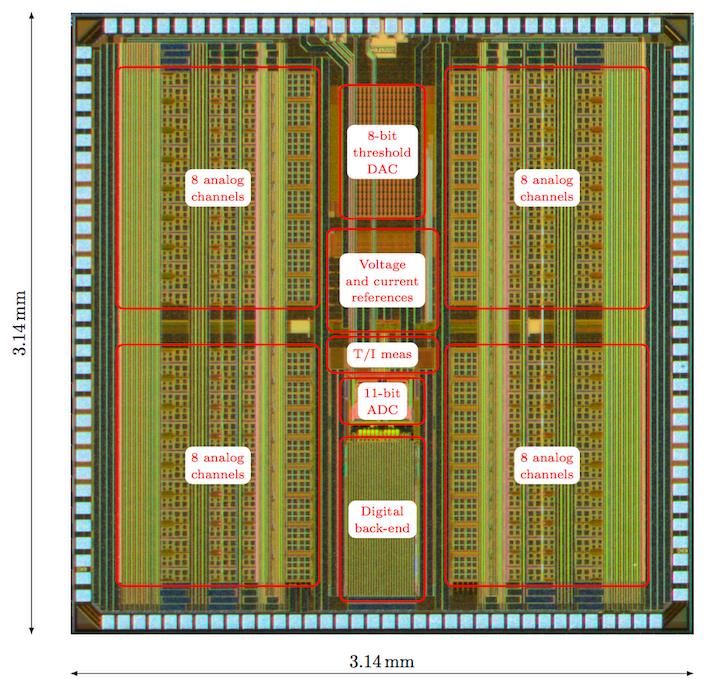
\includegraphics[height=0.5\textheight]{images/experiment_intro/gaps_asic_circuit.jpg}
        \end{figure}
    \end{columns}
\end{frame}


\begin{frame}{Dynamic Signal Compression}
    \fontsize{8.5pt}{1}\selectfont
    \settowidth{\leftmargini}{\usebeamertemplate{itemize item}}
    \addtolength{\leftmargini}{\labelsep}

    \begin{columns}
        \column{0.5\textwidth}
            \begin{itemize}
                \item \textbf{Basic Idea}: exploit the non-linear feature of MOS capacitors to change the gain of CSA with the input signal amplitude
                \item It is based on the nonlinear behaviour of a MOSFET capacitor operating in the inversion mode
                \item Suitable choice of \texttt{W} and \texttt{L} to set the gain in the low and high energy regime 
            \end{itemize}

            \centering
            \vspace{0.5cm}
            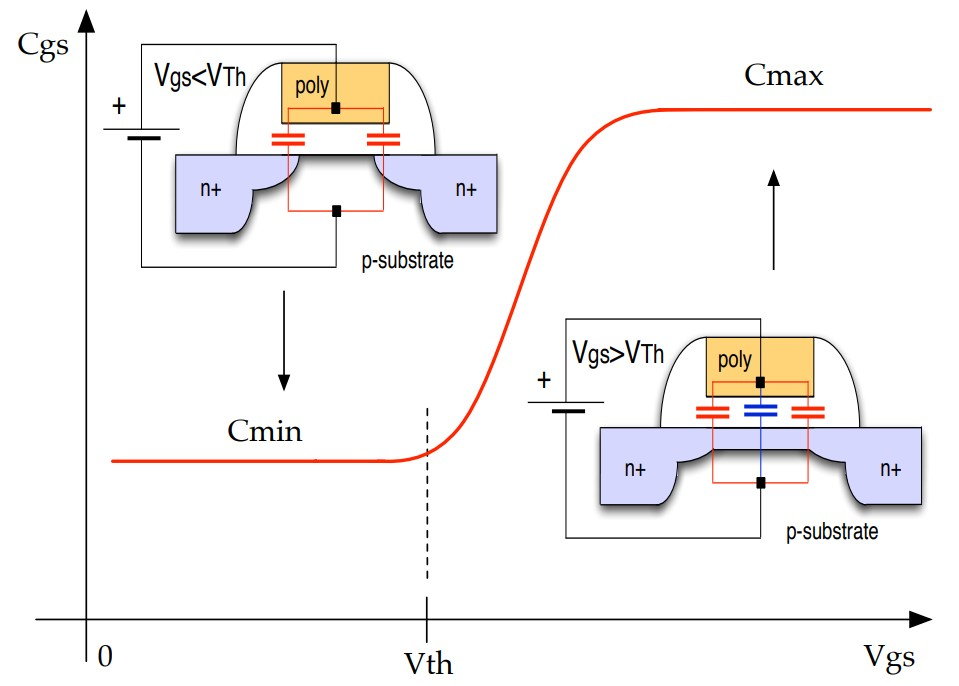
\includegraphics[height=0.5\textheight]{images/backup_slides/capacitance_value_plot.jpg}

        \column{0.5\textwidth}
            \centering
            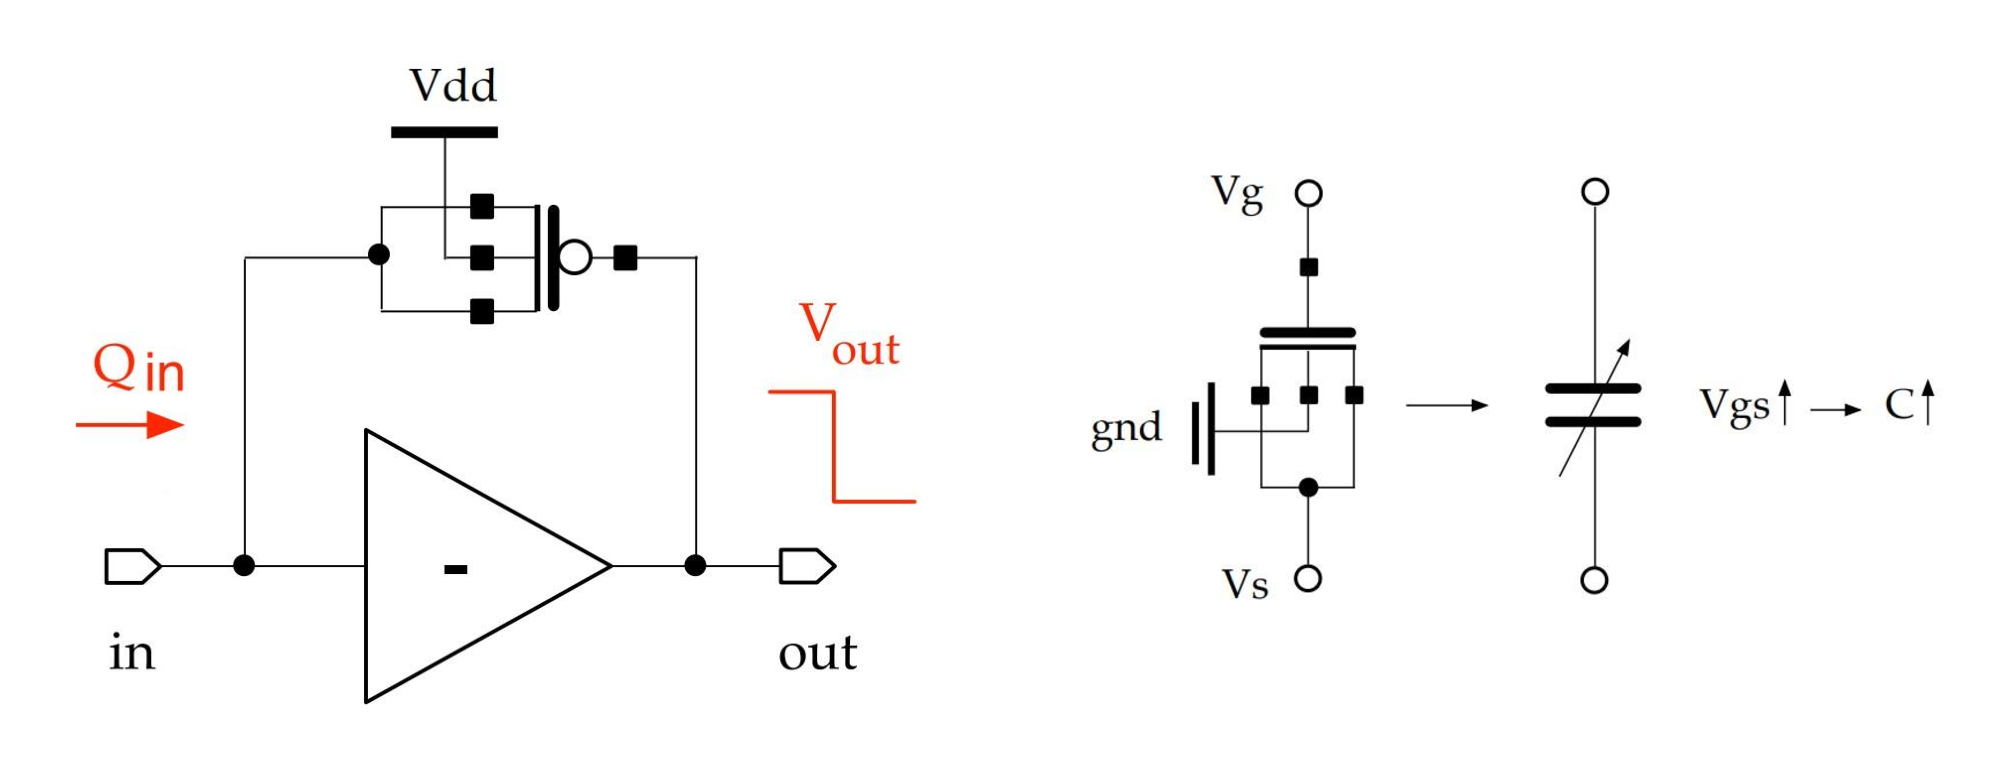
\includegraphics[width=0.9\textwidth]{images/backup_slides/dynamic_compression.pdf}

            \vspace{0.2cm}
            \begin{itemize}
                \item $0 < V_{GS} \ll V_{Th} \rightarrow C_{GS}$ is set at its minimum and it is mainly due to the overlap gate-to-source $C_{GS,ov}$ and gate-to-drain $C_{GD, ov}$ capacitances:
                \begin{equation*}
                    C_{min} \approx C_{GS,ov} + C_{GD,ov} = 2W\Delta L C_{OX}
                \end{equation*}
                \item $V_{GS} \gg V_{Th} \rightarrow C_{GS}$ shows a maximum value which is mainly given by the gate-to-channel $C_{GC}$ capacitance:
                \begin{equation*}
                    C_{max} \approx C_{GC} = WLC_{OX}
                \end{equation*}
            \end{itemize}

            \vspace{-0.25cm}
            \begin{equation*}
                Gain \propto \frac{1}{C_{f}}
            \end{equation*}
            
    \end{columns}
    
\end{frame}

\begin{frame}{Front-end and Flex-rigid boards}
    \fontsize{8.5pt}{1}\selectfont
    \settowidth{\leftmargini}{\usebeamertemplate{itemize item}}
    \addtolength{\leftmargini}{\labelsep}

    \begin{columns}
        \column{0.45\textwidth}
            \vskip0.1cm
            \fontsize{9.5pt}{1}\selectfont
            \textbf{\textcolor{Red}{Front-end board}}
            \fontsize{8.5pt}{1}\selectfont
            \begin{itemize}
                \setlength\itemsep{0.2em}
                \item One ASIC connected to 4 Si(Li) detectors
                \vspace{-0.15cm}
                \item Voltage regulators and filtering for
                    \begin{itemize}
                        \fontsize{8.5pt}{1}\selectfont
                        \item Si(Li) detector High Voltage Power Supply
                        \item ASIC Low Voltage Power Supply (AVDD, DVDD)
                    \end{itemize}
                \item ASIC SPI control signals
                \item ADC clock
                \item Temperature sensor
                \item ASIC calibration system (16 bit DAC)
            \end{itemize}

            \vspace{0.1cm}
            \fontsize{9.5pt}{1}\selectfont
            \textbf{\textcolor{Red}{Flex-rigid board}}
            \fontsize{8.5pt}{1}\selectfont
            \begin{itemize}
                \setlength\itemsep{0.2em}
                \item Connects Front-end boards in series
                \vspace{-0.15cm}
                \item Propagates
                    \begin{itemize}
                        \fontsize{8.5pt}{1}\selectfont
                        \item ASIC Low Voltage Power Supply
                        \item SPI control signals and ADC clock
                    \end{itemize}
            \end{itemize}

            \centering
            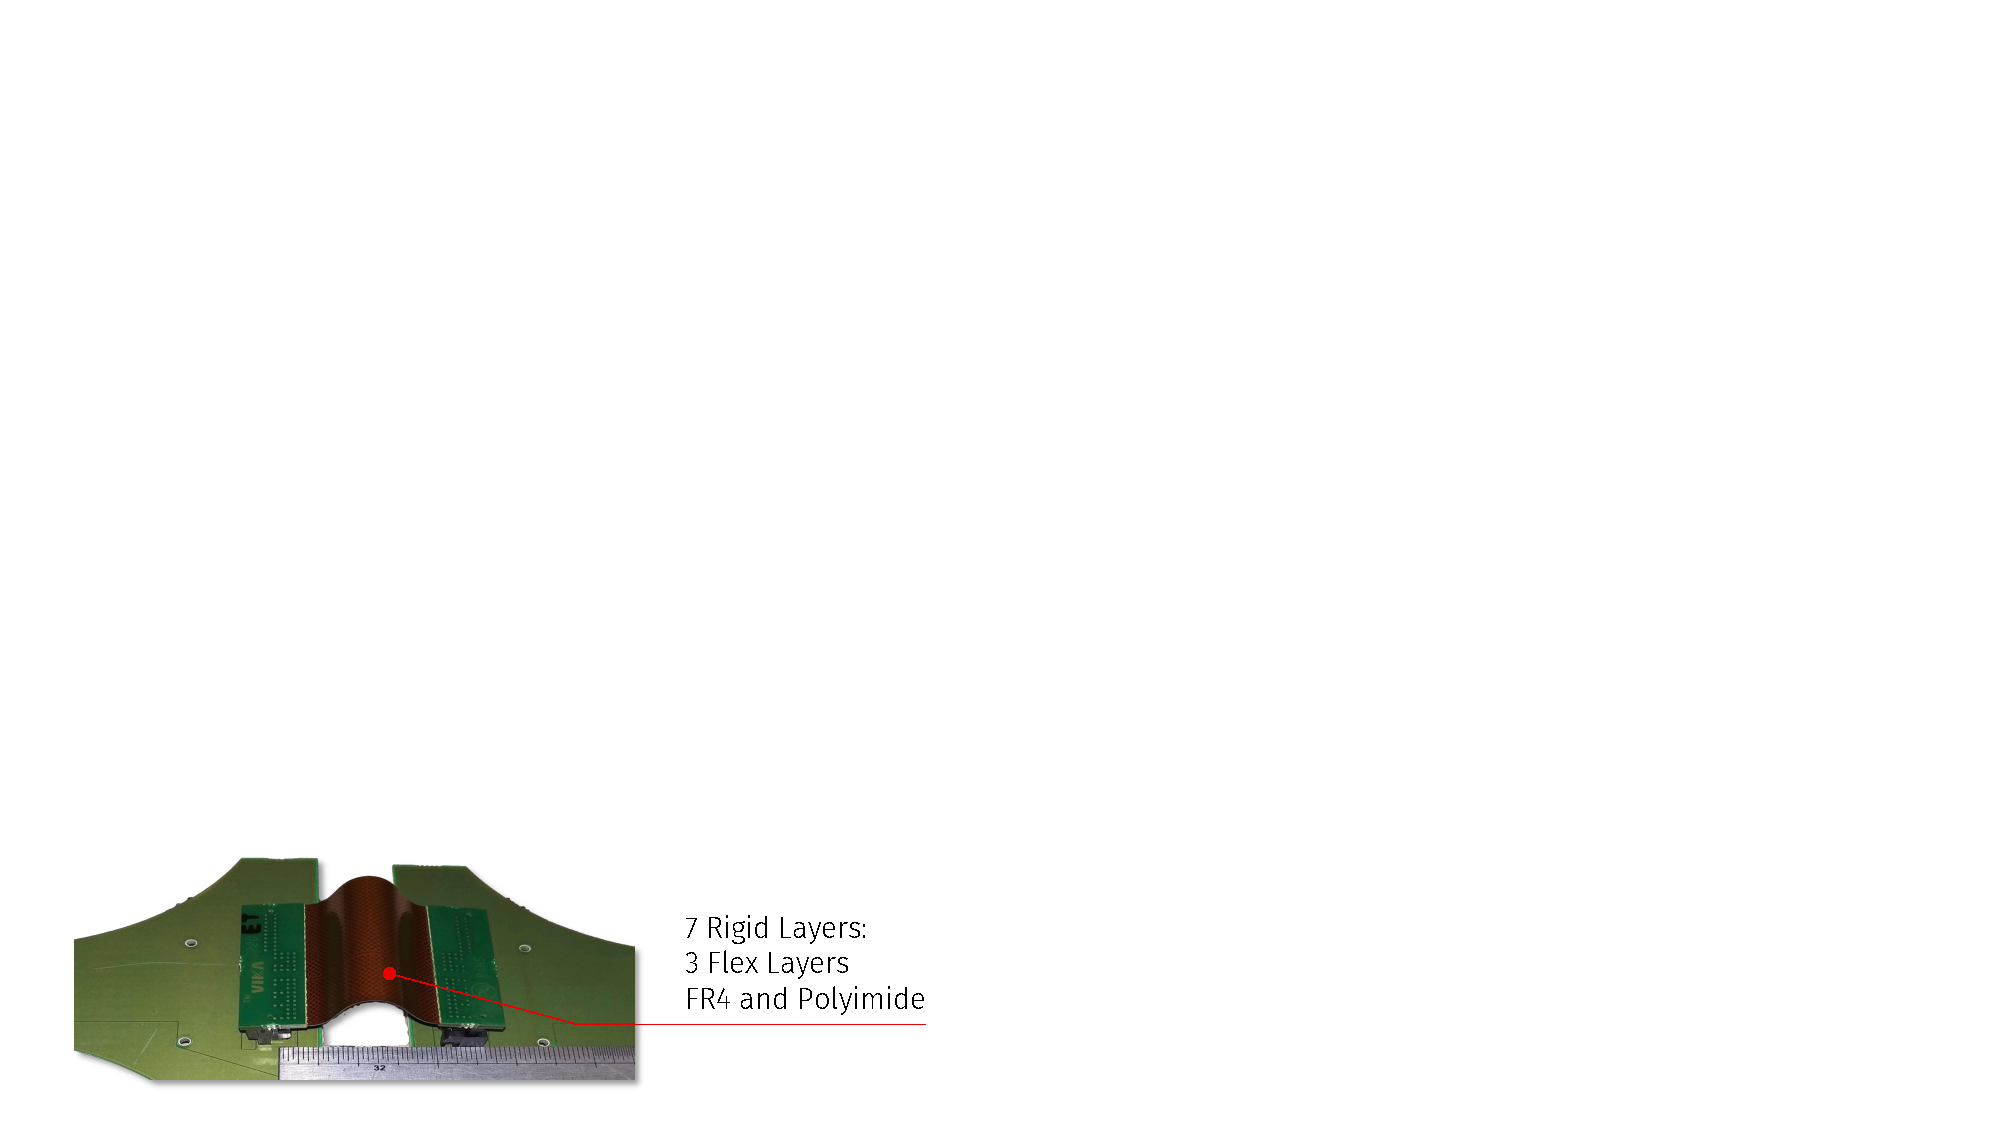
\includegraphics[width=0.97\textwidth]{images/backup_slides/flex_rigid_description.pdf}
          
        \column{0.5\textwidth}
            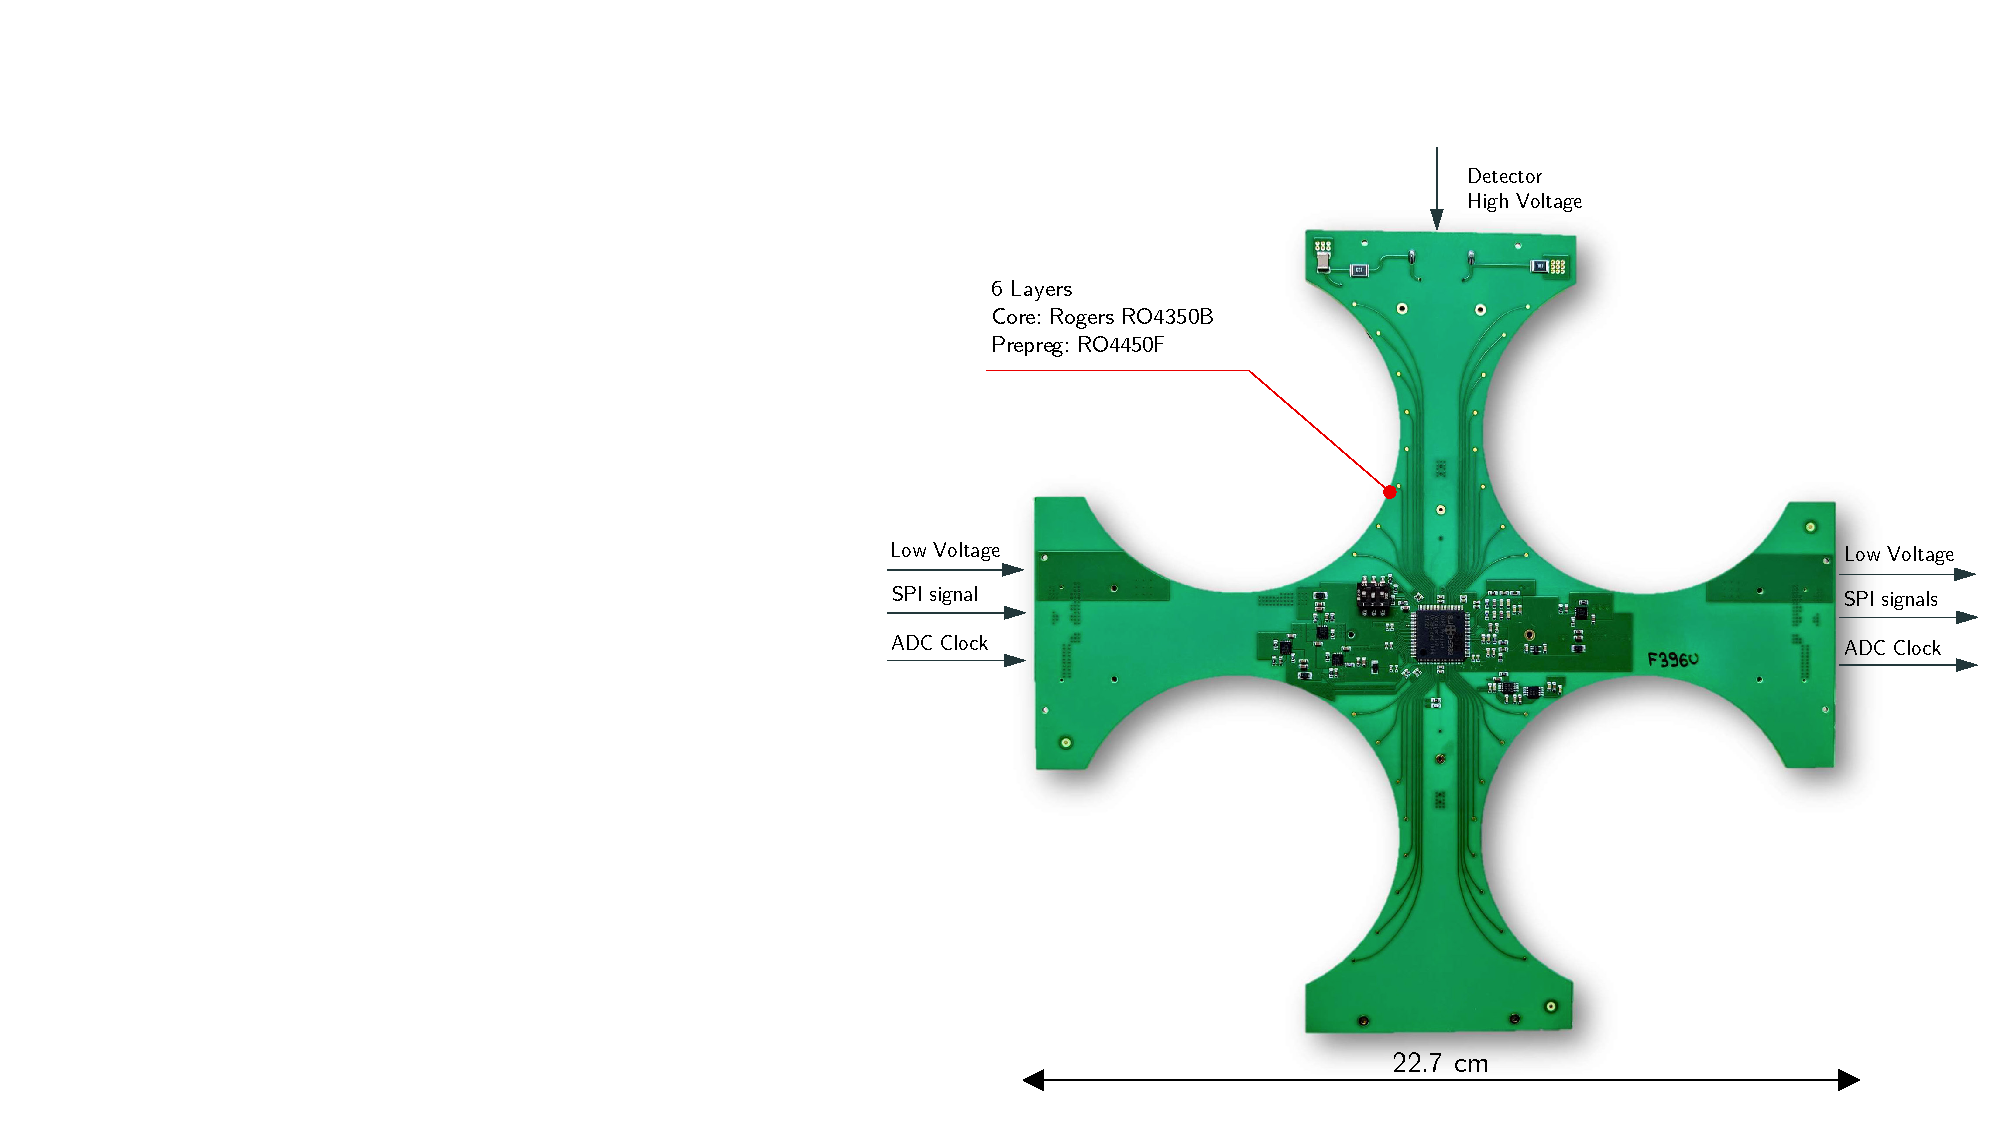
\includegraphics[width=1.05\textwidth]{images/backup_slides/feb_signals.pdf}
            \vspace{-0.5cm}
            
    \end{columns}
    
\end{frame}

\backupend

\end{document}